% !TeX root=../main.tex

\chapter{پاسخ سوالات سری دوم}

% دستور زیر باعث عدم‌نمایش شماره صفحه در اولین صفحهٔ این فصل می‌شود.
%\thispagestyle{empty}
\section{ پاسخ سوال 1}
\section{سوال اول}


یک سیستم خطی با مدل زیر در نظر گرفته می‌شود:  
\[
x(k+1) = A x(k) + B u(k),
\]
که در آن:
\[
A = \begin{bmatrix} 1 & 0 \\ 1 & 1 \end{bmatrix}, \quad B = \begin{bmatrix} 1 \\ 1 \end{bmatrix}.
\]

هدف این است که تابع هزینه زیر را کمینه کنیم:
\[
J = \|x(N)\|^2 + 2 \sum_{i=0}^{N-1} \|u(i)\|^2.
\]

محدودیت‌های سیستم به صورت زیر است:
\[
|x(k)| \leq \begin{bmatrix} 0.5 \\ 0.5 \end{bmatrix}, \quad |u(k)| \leq 0.5.
\]

سطح کوانتیزه‌سازی برای حالت و ورودی هر دو برابر با ۰.۵ در نظر گرفته شده است.

\subsection*{روش حل }
برای حل این مسئله از روش برنامه‌ریزی دینامیک به صورت گسسته استفاده می‌کنیم. در این روش، از مرحله نهایی به مرحله اولیه به صورت معکوس حرکت می‌کنیم و در هر مرحله، ورودی‌های کنترلی بهینه را مشخص می‌کنیم. این روش شامل محاسبه تابع هزینه در هر مرحله و یافتن ورودی کنترلی است که تابع هزینه را کمینه کند.  
ما از مرحله \( k = N-1 \) تا \( k = 0 \) به صورت معکوس حرکت می‌کنیم. تابع هزینه در هر مرحله \( k \) به صورت زیر تعریف می‌شود:
\[
J_k(x(k)) = \min_{u(k)} \left( J_{k+1}(x(k+1)) + 2\|u(k)\|^2 \right),
\]
که در آن \( x(k+1) = A x(k) + B u(k) \).

این فرمول، هزینه آینده \( J_{k+1}(x(k+1)) \) و هزینه کنترلی در لحظه \( 2\|u(k)\|^2 \) را ترکیب می‌کند. هدف یافتن ورودی کنترلی \( u(k) \) است که این هزینه را در هر مرحله کمینه کند.

\subsection*{مرحله \( k = 1 \): محاسبه معکوس}
تابع هزینه در مرحله \( k = 1 \) به صورت زیر است:
\[
J_1(x(1)) = \min_{u(1)} \left( \|x(2)\|^2 + 2\|u(1)\|^2 \right),
\]
که در آن:
\[
x(2) = A x(1) + B u(1).
\]

مقادیر کوانتیزه ممکن عبارتند از:
\begin{itemize}
	\item \( x(1) \in \{-0.5, 0, 0.5\} \)
	\item \( u(1) \in \{-0.5, 0, 0.5\} \)
\end{itemize}

سطح کوانتیزه‌سازی مسئله را ساده‌تر می‌کند و تعداد مقادیر ممکن برای حالت و ورودی را محدود می‌کند. همچنین با کوچک کردن ناحیه جستجو، اجازه می‌دهد تا همه سناریوهای مختلف را بررسی کنیم.

\subsection*{محاسبات مربوط به مرحله \( k = 1 \)}
\begin{itemize}
	\item برای \( x(1) = 0.5 \) و \( u(1) = -0.5 \):
	\[
	x(2) = A \begin{bmatrix} 0.5 \\ 0.5 \end{bmatrix} + B(-0.5) = \begin{bmatrix} 0 \\ 0.5 \end{bmatrix}, \quad \|x(2)\|^2 = 0.25, \quad 2\|u(1)\|^2 = 0.5.
	\]
	هزینه نهایی: \( J_1(0.5) = 0.75 \).
	
	\item برای \( x(1) = 0.5 \) و \( u(1) = 0 \):
	\[
	x(2) = A \begin{bmatrix} 0.5 \\ 0.5 \end{bmatrix} + B(0) = \begin{bmatrix} 0.5 \\ 0.5 \end{bmatrix}, \quad \|x(2)\|^2 = (0.5)^2 + (0.5)^2 = 0.5.
	\]
	هزینه نهایی: \( J_1(0.5) = 0.5 \).
	
	\item برای \( x(1) = 0 \) و \( u(1) = -0.5 \):
	\[
	x(2) = A \begin{bmatrix} 0 \\ 0 \end{bmatrix} + B(-0.5) = \begin{bmatrix} -0.5 \\ -0.5 \end{bmatrix}, \quad \|x(2)\|^2 = (0.5)^2 + (0.5)^2 = 0.5, 
	\]
	\[
	2\|u(1)\|^2 = 0.5.
	\]
	هزینه نهایی: \( J_1(0) = 1 \).
	
	\item برای \( x(1) = -0.5 \) و \( u(1) = 0.5 \):
	\[
	x(2) = A \begin{bmatrix} -0.5 \\ -0.5 \end{bmatrix} + B(0.5) = \begin{bmatrix} 0 \\ -0.5 \end{bmatrix}, \quad \|x(2)\|^2 = 0.25, \quad 2\|u(1)\|^2 = 0.5.
	\]
	هزینه نهایی: \( J_1(-0.5) = 0.75 \).
\end{itemize}

	\subsection*{محاسبات مربوط به مرحله \( k = 1 \)}
\begin{itemize}
	\item[-] برای \( x(1) = 0.5 \) و \( u(1) = -0.5 \):
	\[
	x(2) = A \begin{bmatrix} 0.5 \\ 0.5 \end{bmatrix} + B(-0.5) = \begin{bmatrix} 0 \\ 0.5 \end{bmatrix}, \quad \|x(2)\|^2 = 0.25, \quad 2\|u(1)\|^2 = 2(0.5)^2 = 0.5.
	\]
	هزینه نهایی: \( J_1(0.5) = 0.75 \).\\
	
	\item[-] برای \( x(1) = 0.5 \) و \( u(1) = 0 \):
	\[
	x(2) = A \begin{bmatrix} 0.5 \\ 0.5 \end{bmatrix} + B(0) = \begin{bmatrix} 0.5 \\ 0.5 \end{bmatrix}, \quad \|x(2)\|^2 = (0.5)^2 + (0.5)^2 = 0.5.
	\]
	هزینه نهایی: \( J_1(0.5) = 0.5 \).\\
	
	\item[-] برای \( x(1) = 0 \) و \( u(1) = -0.5 \):
	\[
	x(2) = A \begin{bmatrix} 0 \\ 0 \end{bmatrix} + B(-0.5) = \begin{bmatrix} -0.5 \\ -0.5 \end{bmatrix}, \quad \|x(2)\|^2 = (0.5)^2 + (0.5)^2 = 0.5, 
	\]
	\[
	\quad 2\|u(1)\|^2 = 0.5.
	\]
	هزینه نهایی: \( J_1(0) = 1 \).\\
	
	
	
	
	\item[-] برای \( x(1) = -0.5 \) و \( u(1) = 0.5 \):
	\[
	x(2) = A \begin{bmatrix} -0.5 \\ -0.5 \end{bmatrix} + B(0.5) = \begin{bmatrix} 0 \\ -0.5 \end{bmatrix}, \quad \|x(2)\|^2 = 0.25, \quad 2\|u(1)\|^2 = 0.5.
	\]
	هزینه نهایی: \( J_1(-0.5) = 0.75 \).
\end{itemize}
\subsection*{جدول محاسبات پویا برای \( k = 1 \)}
\begin{latin}
	\begin{longtable}{|c|c|c|c|c|c|}
		\hline
		\rowcolor[HTML]{00D2CB} 
		& 	 & 	 & $J$ &	 &	\\
		\rowcolor[HTML]{00D2CB} 
		\multirow{-2}{*}{$x(1)$}	&\multirow{-2}{*}{$u(1)$ }	&\multirow{-2}{*}{$x(2)$}	& $J_{k+1}(x(k+1)) + 2\|u(k)\|^2$ &\multirow{-2}{*}{$J^*$}	& \multirow{-2}{*}{$u^*(1)$}\\ \hline
		\endfirsthead                                                 
		%
		\endhead
		%
		&-0.5&$\begin{bmatrix} 0 \\ 0.5 \end{bmatrix}$&0.75&	&	\\  \cline{2-4} 
		\multirow{-3}{*}{$\begin{bmatrix} 0.5 \\ 0.5 \end{bmatrix}$}&0&$\begin{bmatrix} 0.5 \\ 1 \end{bmatrix}$&Infeasible&0.75&-0.5	\\  \cline{2-4} 		
		&0.5&$\begin{bmatrix} 1 \\ 1.5 \end{bmatrix}$&Infeasible&	&	\\  \cline{2-4} \hline
		
		&      -0.5                  &$\begin{bmatrix} 0 \\ 0 \end{bmatrix}$      &     0.5 &             &   \\  \cline{2-4} 
		\multirow{-3}{*}{$\begin{bmatrix} 0.5 \\ 0 \end{bmatrix}$}&        0                &$\begin{bmatrix} 0.5 \\ 0.5 \end{bmatrix}$      &      0.5                  &    0.5     &  $\{-0.5,0\}$   \\  \cline{2-4} 
		&         -0.5               &$\begin{bmatrix} 1 \\ 1 \end{bmatrix}$      & Infeasible                        &              &   \\  \cline{2-4} \hline
		
		& -0.5 &$\begin{bmatrix} 0 \\ -0.5 \end{bmatrix}$      &      0.75     &        &         \\ \cline{2-4}
		\multirow{-3}{*}{$\begin{bmatrix} 0.5 \\ -0.5 \end{bmatrix}$}& 0   &$\begin{bmatrix} 0.5 \\ 0 \end{bmatrix}$      &       0.25                 &      0.25       &  0  \\ \cline{2-4}
		& 0.5  &$\begin{bmatrix} 1 \\ 0.5 \end{bmatrix}$      & Infeasible                        &   &                \\	\cline{2-4} \hline
		
		&            -0.5            &$\begin{bmatrix} -0.5 \\ 0 \end{bmatrix}$      &     0.75             &         &         \\  \cline{2-4} 
		\multirow{-3}{*}{$\begin{bmatrix} 0 \\ 0.5 \end{bmatrix}$}&        0                &$\begin{bmatrix} 0 \\ 0.5 \end{bmatrix}$      &      0.25                  &  0.25            &  0  \\  \cline{2-4} 
		&           0.5             &$\begin{bmatrix} 0.5 \\ 1 \end{bmatrix}$      & Infeasible                        &          &  \\  \cline{2-4} \hline
		
		&          -0.5              &$\begin{bmatrix} -0.5 \\ -0.5 \end{bmatrix}$      &        1             &      &        \\  \cline{2-4} 
		\multirow{-3}{*}{$\begin{bmatrix} 0 \\ 0 \end{bmatrix}$}&       0                 &$\begin{bmatrix} 0 \\ 0 \end{bmatrix}$      &     0                   &        0        &0  \\  \cline{2-4} 
		&           0.5             &$\begin{bmatrix} 0.5 \\ 0.5 \end{bmatrix}$      &             1            &           &  \\  \cline{2-4} \hline
		
		& -0.5 &$\begin{bmatrix} -0.5 \\ -1 \end{bmatrix}$      & Infeasible                        &             &      \\ \cline{2-4}
		\multirow{-3}{*}{$\begin{bmatrix} 0 \\ -0.5 \end{bmatrix}$}& 0    &$\begin{bmatrix} 0 \\ -0.5 \end{bmatrix}$      &     0.25                   &    0.25        &  0     \\ \cline{2-4}
		& 0.5  &$\begin{bmatrix} 0.5 \\ 0 \end{bmatrix}$      &    0.75                     &          &       \\ \hline
		
		&          -0.5              &$\begin{bmatrix} -1 \\ -0.5 \end{bmatrix}$      & Infeasible                        &       &          \\  \cline{2-4} 
		\multirow{-3}{*}{$\begin{bmatrix} -0.5 \\ 0.5 \end{bmatrix}$}&     0                   &$\begin{bmatrix} -0.5 \\ 0 \end{bmatrix}$      &     0.25                   &  0.25           &   0    \\  \cline{2-4} 
		&         0.5               &$\begin{bmatrix} 0 \\ 0.5 \end{bmatrix}$      &        0.75                    &          &      \\  \cline{2-4} \hline
		
		&              -0.5          &$\begin{bmatrix} -1 \\ -1 \end{bmatrix}$      & Infeasible                        &      &     \\  \cline{2-4} 
		\multirow{-3}{*}{$\begin{bmatrix} -0.5 \\ 0 \end{bmatrix}$}&      0                  &$\begin{bmatrix} -0.5 \\ 0 \end{bmatrix}$      &      0.25                  &  0.25          &     0   \\  \cline{2-4} 
		&              0.5          &$\begin{bmatrix} 0 \\ 0.5 \end{bmatrix}$      &    0.75                &                 &     \\  \cline{2-4} \hline	
		
		& -0.5 &$\begin{bmatrix} -1 \\ -1.5 \end{bmatrix}$      & Infeasible                        &            &        \\ \cline{2-4}
		\multirow{-3}{*}{$\begin{bmatrix} -0.5 \\ -0.5 \end{bmatrix}$}& 0   &$\begin{bmatrix} 0 \\ -1 \end{bmatrix}$      & Infeasible                        &    0.75       &  0.5	      \\ \cline{2-4}
		& 0.5 &$\begin{bmatrix} 0 \\ -0.5 \end{bmatrix}$      &    0.75                    &                &      \\ \hline
		
	\end{longtable}
\end{latin}

	\newpage
\subsection*{جدول محاسبات پویا برای \( k = 0 \)}
\begin{latin}
	\begin{longtable}{|c|c|c|c|c|c|}
		\hline
		\rowcolor[HTML]{00D2CB} 
		& 	 & 	 & $J$ &	 &	\\
		\rowcolor[HTML]{00D2CB} 
		\multirow{-2}{*}{$x(1)$}	&\multirow{-2}{*}{$u(1)$ }	&\multirow{-2}{*}{$x(2)$}	& $J_{k+1}(x(k+1)) + 2\|u(k)\|^2$ &\multirow{-2}{*}{$J^*$}	& \multirow{-2}{*}{$u^*(1)$}\\ \hline
		\endfirsthead                                             
		%
		\endhead
		%
		&-0.5&$\begin{bmatrix} 0 \\ 0.5 \end{bmatrix}$&1.25&	&	\\  \cline{2-4} 
		\multirow{-3}{*}{$\begin{bmatrix} 0.5 \\ 0.5 \end{bmatrix}$}&0&$\begin{bmatrix} 0.5 \\ 1 \end{bmatrix}$&Infeasible&1.25&-0.5	\\  \cline{2-4} 		
		&0.5&$\begin{bmatrix} 1 \\ 1.5 \end{bmatrix}$&Infeasible&	&	\\  \cline{2-4} \hline
		
		&      -0.5                  &$\begin{bmatrix} 0 \\ 0 \end{bmatrix}$      &    1 &             &   \\  \cline{2-4} 
		\multirow{-3}{*}{$\begin{bmatrix} 0.5 \\ 0 \end{bmatrix}$}&        0                &$\begin{bmatrix} 0.5 \\ 0.5 \end{bmatrix}$      &      0.5                  &    0.5     &  $0$   \\  \cline{2-4} 
		&         -0.5               &$\begin{bmatrix} 1 \\ 1 \end{bmatrix}$      & Infeasible                        &              &   \\  \cline{2-4} \hline
		
		& -0.5 &$\begin{bmatrix} 0 \\ -0.5 \end{bmatrix}$      &      1.25     &        &         \\ \cline{2-4}
		\multirow{-3}{*}{$\begin{bmatrix} 0.5 \\ -0.5 \end{bmatrix}$}& 0   &$\begin{bmatrix} 0.5 \\ 0 \end{bmatrix}$      &       0.25                 &      0.25       &  0  \\ \cline{2-4}
		& 0.5  &$\begin{bmatrix} 1 \\ 0.5 \end{bmatrix}$      & Infeasible                        &   &                \\	\cline{2-4} \hline
		
		&            -0.5            &$\begin{bmatrix} -0.5 \\ 0 \end{bmatrix}$      &     1.25             &         &         \\  \cline{2-4} 
		\multirow{-3}{*}{$\begin{bmatrix} 0 \\ 0.5 \end{bmatrix}$}&        0                &$\begin{bmatrix} 0 \\ 0.5 \end{bmatrix}$      &      0.25                  &  0.25            &  0  \\  \cline{2-4} 
		&           0.5             &$\begin{bmatrix} 0.5 \\ 1 \end{bmatrix}$      & Infeasible                        &          &  \\  \cline{2-4} \hline
		
		&          -0.5              &$\begin{bmatrix} -0.5 \\ -0.5 \end{bmatrix}$      &        1.5             &      &        \\  \cline{2-4} 
		\multirow{-3}{*}{$\begin{bmatrix} 0 \\ 0 \end{bmatrix}$}&       0                 &$\begin{bmatrix} 0 \\ 0 \end{bmatrix}$      &     0                   &        0        &0  \\  \cline{2-4} 
		&           0.5             &$\begin{bmatrix} 0.5 \\ 0.5 \end{bmatrix}$      &             1.5            &           &  \\  \cline{2-4} \hline
		
		& -0.5 &$\begin{bmatrix} -0.5 \\ -1 \end{bmatrix}$      & Infeasible                        &             &      \\ \cline{2-4}
		\multirow{-3}{*}{$\begin{bmatrix} 0 \\ -0.5 \end{bmatrix}$}& 0    &$\begin{bmatrix} 0 \\ -0.5 \end{bmatrix}$      &     0.25                   &    0.25        &  0     \\ \cline{2-4}
		& 0.5  &$\begin{bmatrix} 0.5 \\ 0 \end{bmatrix}$      &    1.25                     &          &       \\ \hline
		
		&          -0.5              &$\begin{bmatrix} -1 \\ -0.5 \end{bmatrix}$      & Infeasible                        &       &          \\  \cline{2-4} 
		\multirow{-3}{*}{$\begin{bmatrix} -0.5 \\ 0.5 \end{bmatrix}$}&     0                   &$\begin{bmatrix} -0.5 \\ 0 \end{bmatrix}$      &     0.25                   &  0.25           &   0    \\  \cline{2-4} 
		&         0.5               &$\begin{bmatrix} 0 \\ 0.5 \end{bmatrix}$      &        1.25                    &          &      \\  \cline{2-4} \hline
		
		&              -0.5          &$\begin{bmatrix} -1 \\ -1 \end{bmatrix}$      & Infeasible                        &      &     \\  \cline{2-4} 
		\multirow{-3}{*}{$\begin{bmatrix} -0.5 \\ 0 \end{bmatrix}$}&      0                  &$\begin{bmatrix} -0.5 \\ 0 \end{bmatrix}$      &      0.25                  &  0.25          &     0   \\  \cline{2-4} 
		&              0.5          &$\begin{bmatrix} 0 \\ 0.5 \end{bmatrix}$      &    1.25                &                 &     \\  \cline{2-4} \hline	
		
		& -0.5 &$\begin{bmatrix} -1 \\ -1.5 \end{bmatrix}$      & Infeasible                        &            &        \\ \cline{2-4}
		\multirow{-3}{*}{$\begin{bmatrix} -0.5 \\ -0.5 \end{bmatrix}$}& 0   &$\begin{bmatrix} 0 \\ -1 \end{bmatrix}$      & Infeasible                        &    1.25       &  0.5	      \\ \cline{2-4}
		& 0.5 &$\begin{bmatrix} 0 \\ -0.5 \end{bmatrix}$      &    1.25                    &                &      \\ \hline
		
	\end{longtable}
\end{latin}
\section{پاسخ سوال 2}
\subsection{بخش یکم}
در این بخش، ابتدا لازم است سیستم در محیط سیمولینک پیاده سازی شده و سپس، با قرار دادن کنترلر MPC و تنظیم آن، خروجی ها مطابق با خواسته های مسیئله تعریف شوند. برای این منظور، با جدا کردن عملگرهای دما و رطوبت از یکدیگر و جمع زدن هر دو گروه هم، ورودی مورد نیاز برای کنترلر را تهیه می کنیم. 

\begin{figure}[H]
	\centering
	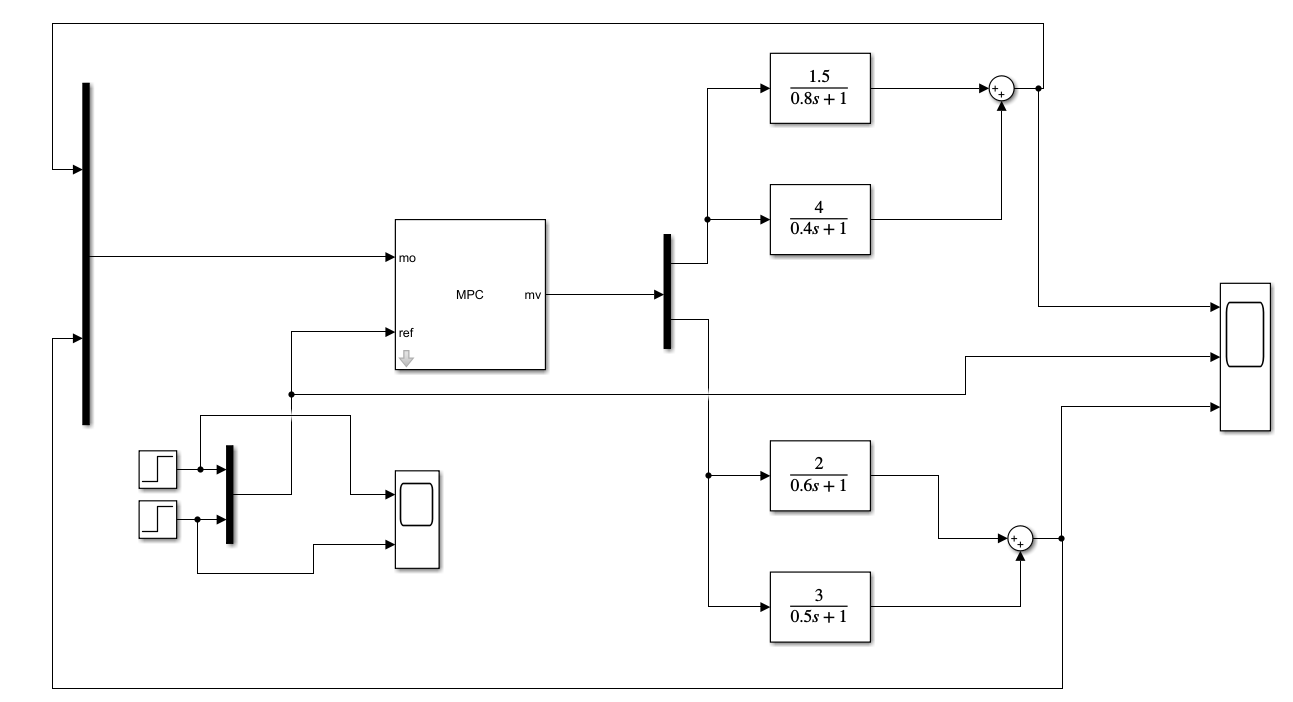
\includegraphics[width=1\linewidth]{../img/Q2_Block_Diagram}
	\caption{بلوک دیاگرام سیستم}
	\label{fig:q2blockdiagram}
\end{figure}

سپس، مقادیر ورودی و رفرنس نیز به وسیله ی بلوک های پله ساخته می شوند.
\begin{figure}[H]
	\centering
	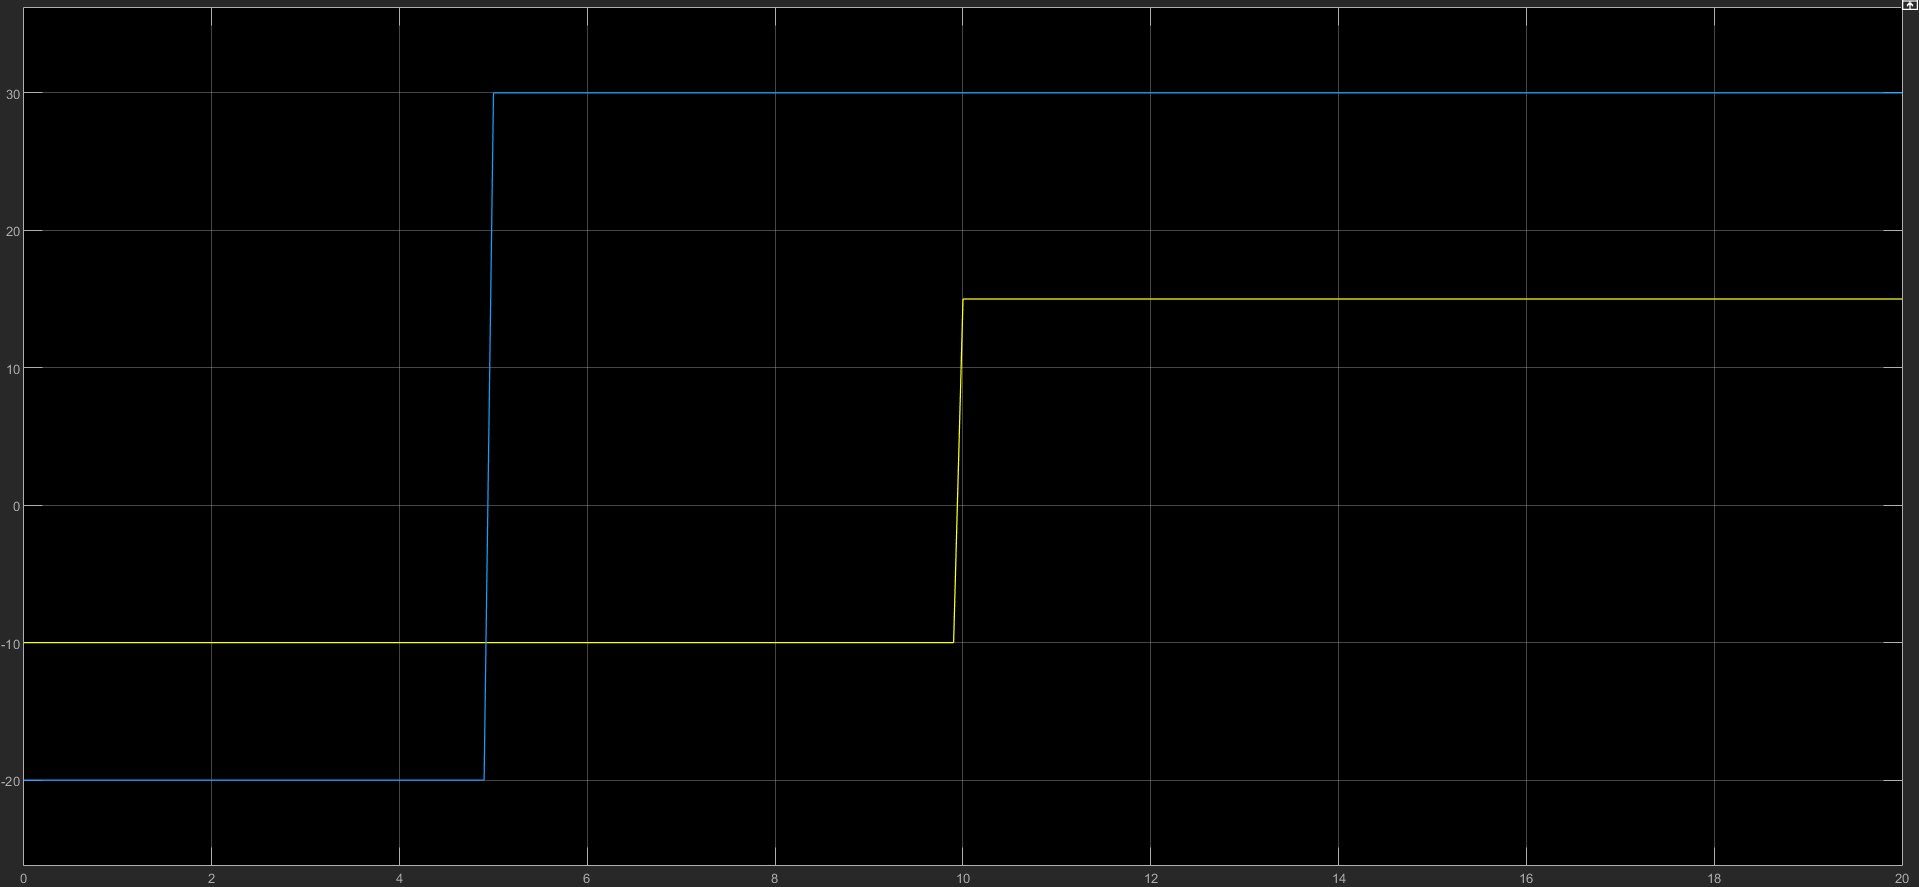
\includegraphics[width=1\linewidth]{../img/Q2_refernece}
	\caption{ورودی های رفرنس}
	\label{fig:q2refernece}
\end{figure}

با سپس، با قرار دادن یک بلوک کنترلر MPC در این سیستم و قرار دادن اسکوپ های مناسب برای بررسی خروجی های سیستم، اقدام به تنظیم پارامترهای کنترلر می کنیم. 
برای این کنترلر، پارامترهای زیر در نظر گرفته شده اند:
\[
\begin{array}{|c|c|}
	\hline
	\textbf{Parameter} & \textbf{Value} \\ 
	\hline
	T_s \, (\text{Sampling Time}) & 0.1 \\ 
	\hline
	\text{Prediction Horizon} & 100 \\ 
	\hline
	\text{Control Horizon} & 20 \\ 
	\hline
\end{array}
\]
همچنین، قید ها و وزن های مطرح شده در سوال نیز برای کنترلر تعریف می شوند.
\begin{figure}[H]
	\centering
	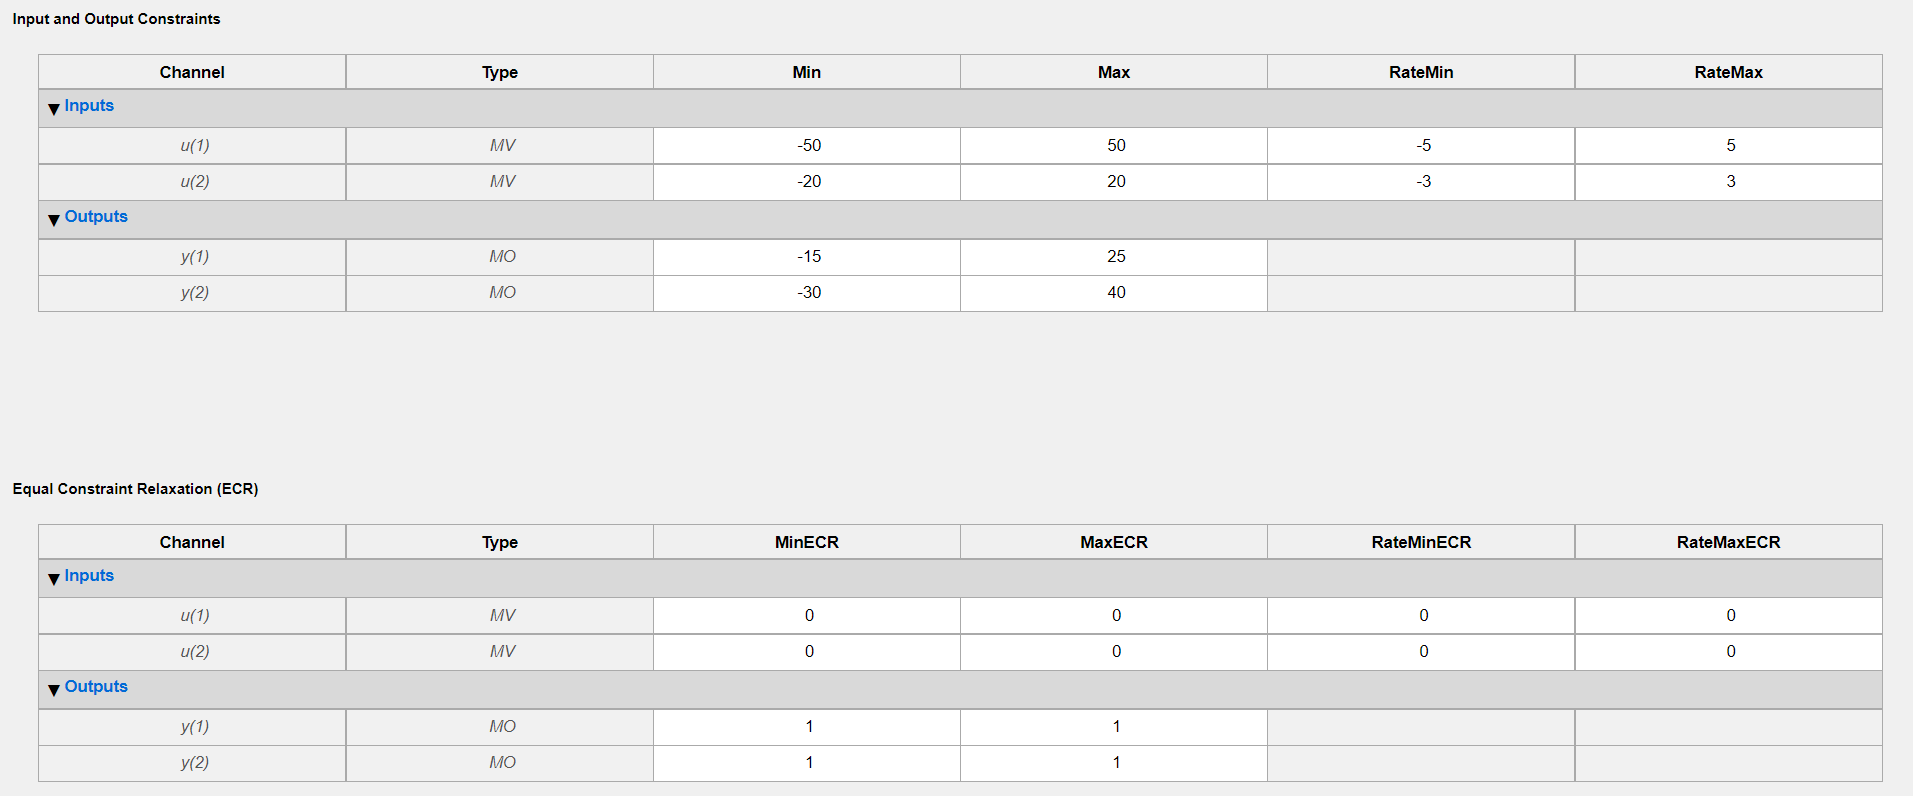
\includegraphics[width=1\linewidth]{../img/Q2_constraints}
	\caption{قیدها}
	\label{fig:q2constraints}
\end{figure}

\begin{figure}[H]
	\centering
	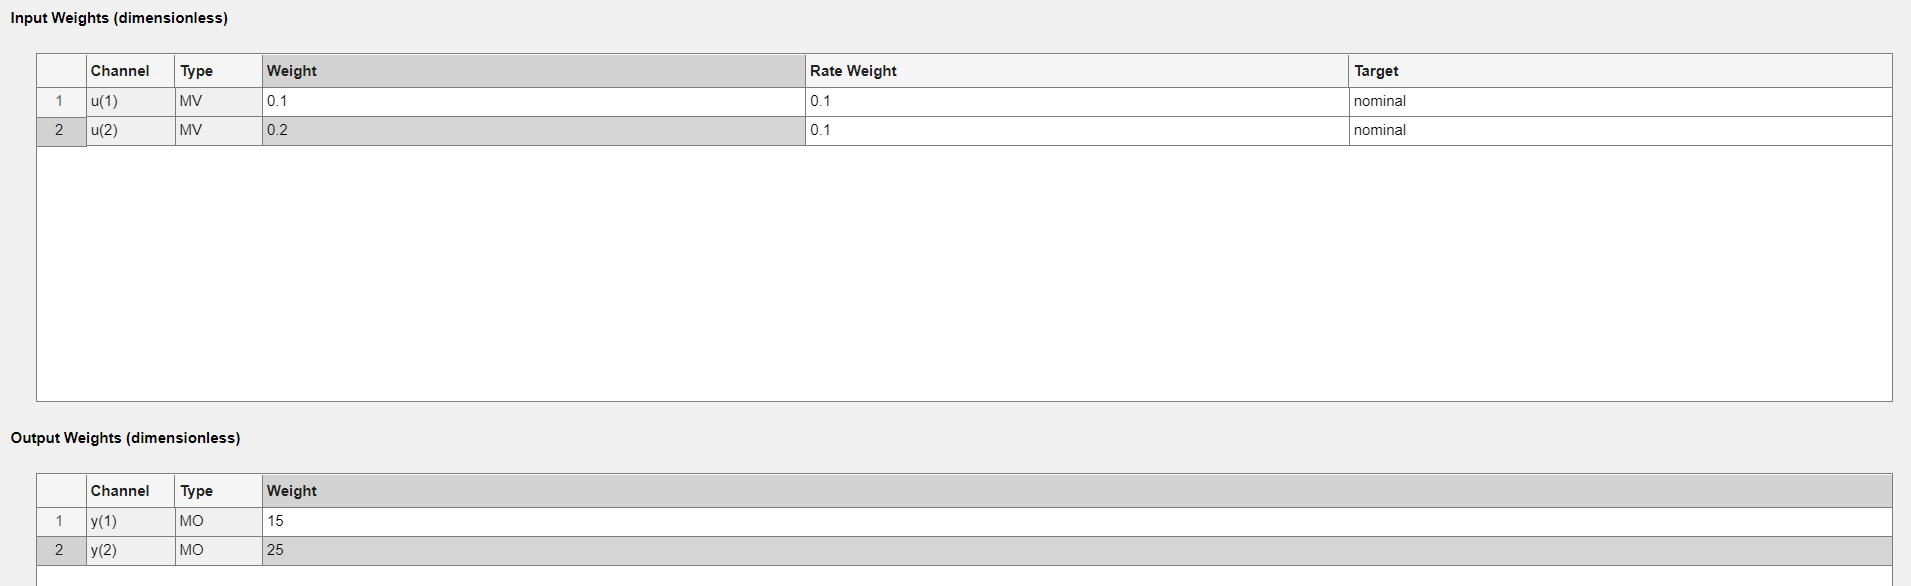
\includegraphics[width=1\linewidth]{../img/Q2_weights}
	\caption{وزن ها}
	\label{fig:q2weights}
\end{figure}

در پایان، با اجرای برنامه مشاهده می شود که کنترلر طراحی شده قادر است با عملکرد مناسبی مقادیر رفرنس را دنبال کنید.
\begin{figure}
	\centering
	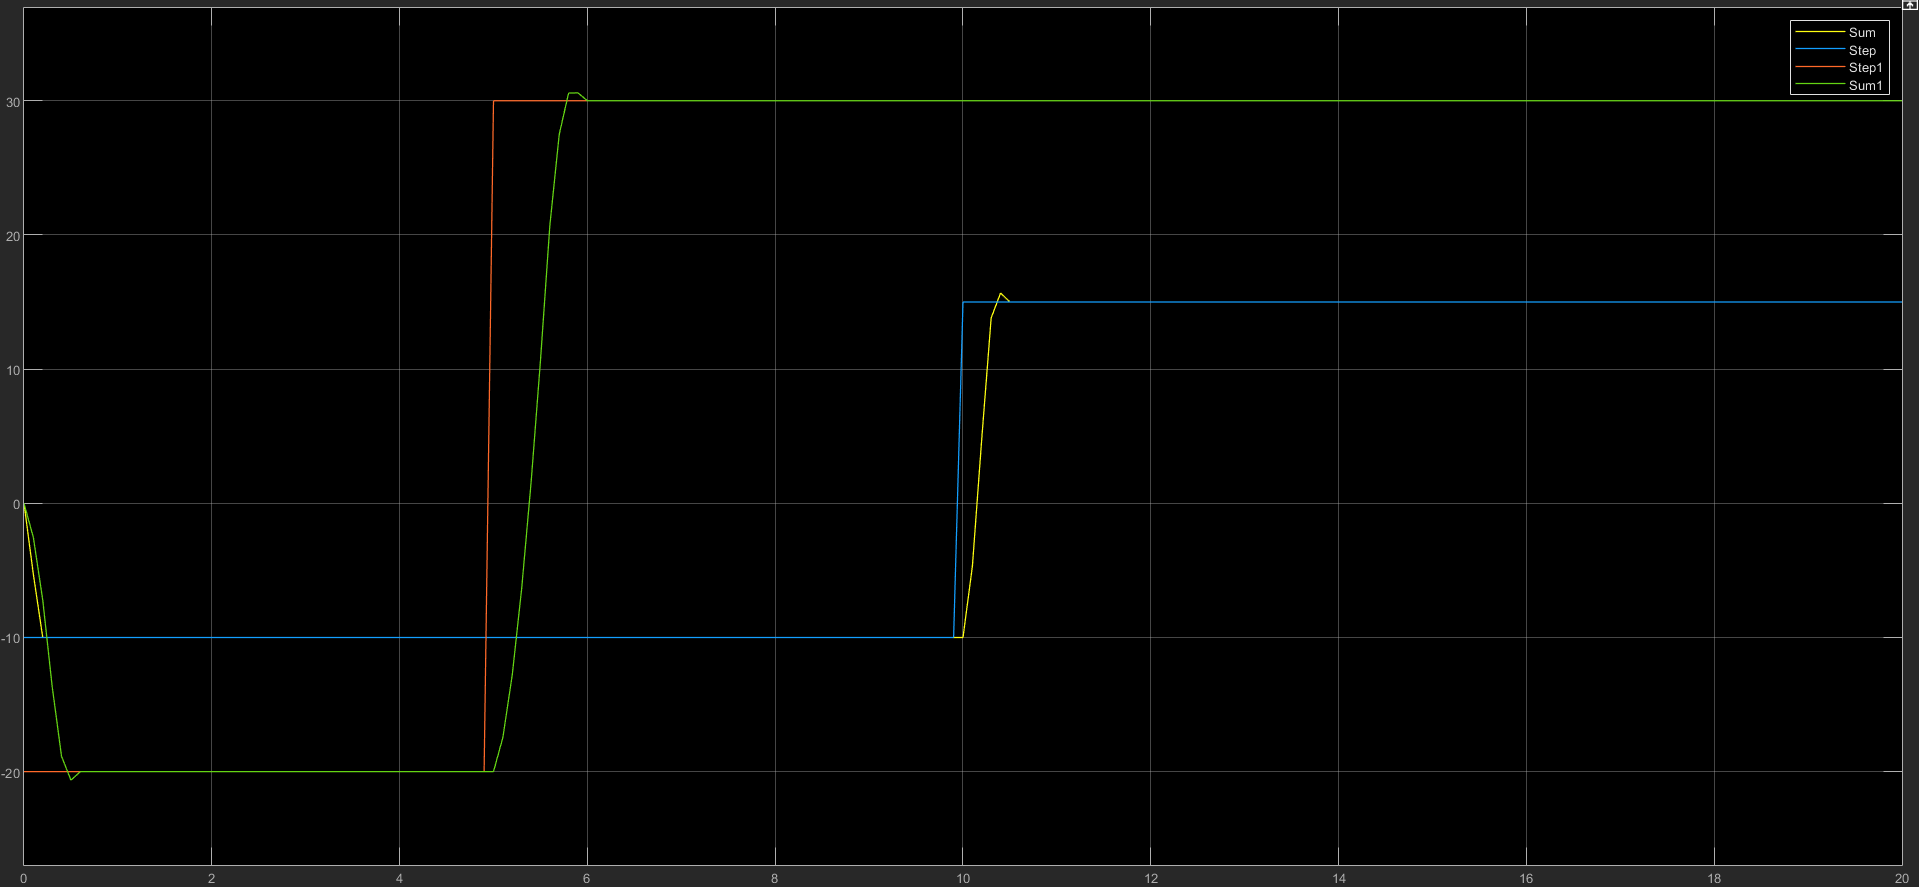
\includegraphics[width=1\linewidth]{../img/Q2_output}
	\caption{پاسخ سیستم}
	\label{fig:q2output}
\end{figure}

\subsection{بخش دوم}
در این بخش، پارامترهای سیستم شامل وزن ها، نرخ نمونه برداری، و افق پیش بین و کنترل را تغییر می دهیم.
\[
\begin{array}{|c|c|}
	\hline
	\textbf{Parameter} & \textbf{Value} \\ 
	\hline
	T_s \, (\text{Sampling Time}) & 0.3 \\ 
	\hline
	\text{Prediction Horizon} & 200 \\ 
	\hline
	\text{Control Horizon} & 40 \\ 
	\hline
\end{array}
\]

 و وزن ها نیز به صورت برابر تغییر داده شده اند:
 \begin{figure}
 	\centering
 	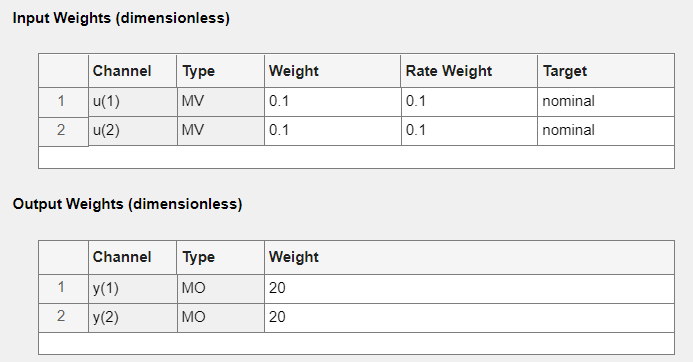
\includegraphics[width=1\linewidth]{../img/Q2_weights_updated}
 	\caption{وزن های تغییر یافته}
 	\label{fig:q2weightsupdated}
 \end{figure}
 
 در این شرایط، مشاهده می کنیم که خروجی های سیستم در مقایسه با حالت اول دارای فراجهش کمتر اما زمان خیزش و نشست بیشتری است.
 \begin{figure}
 	\centering
 	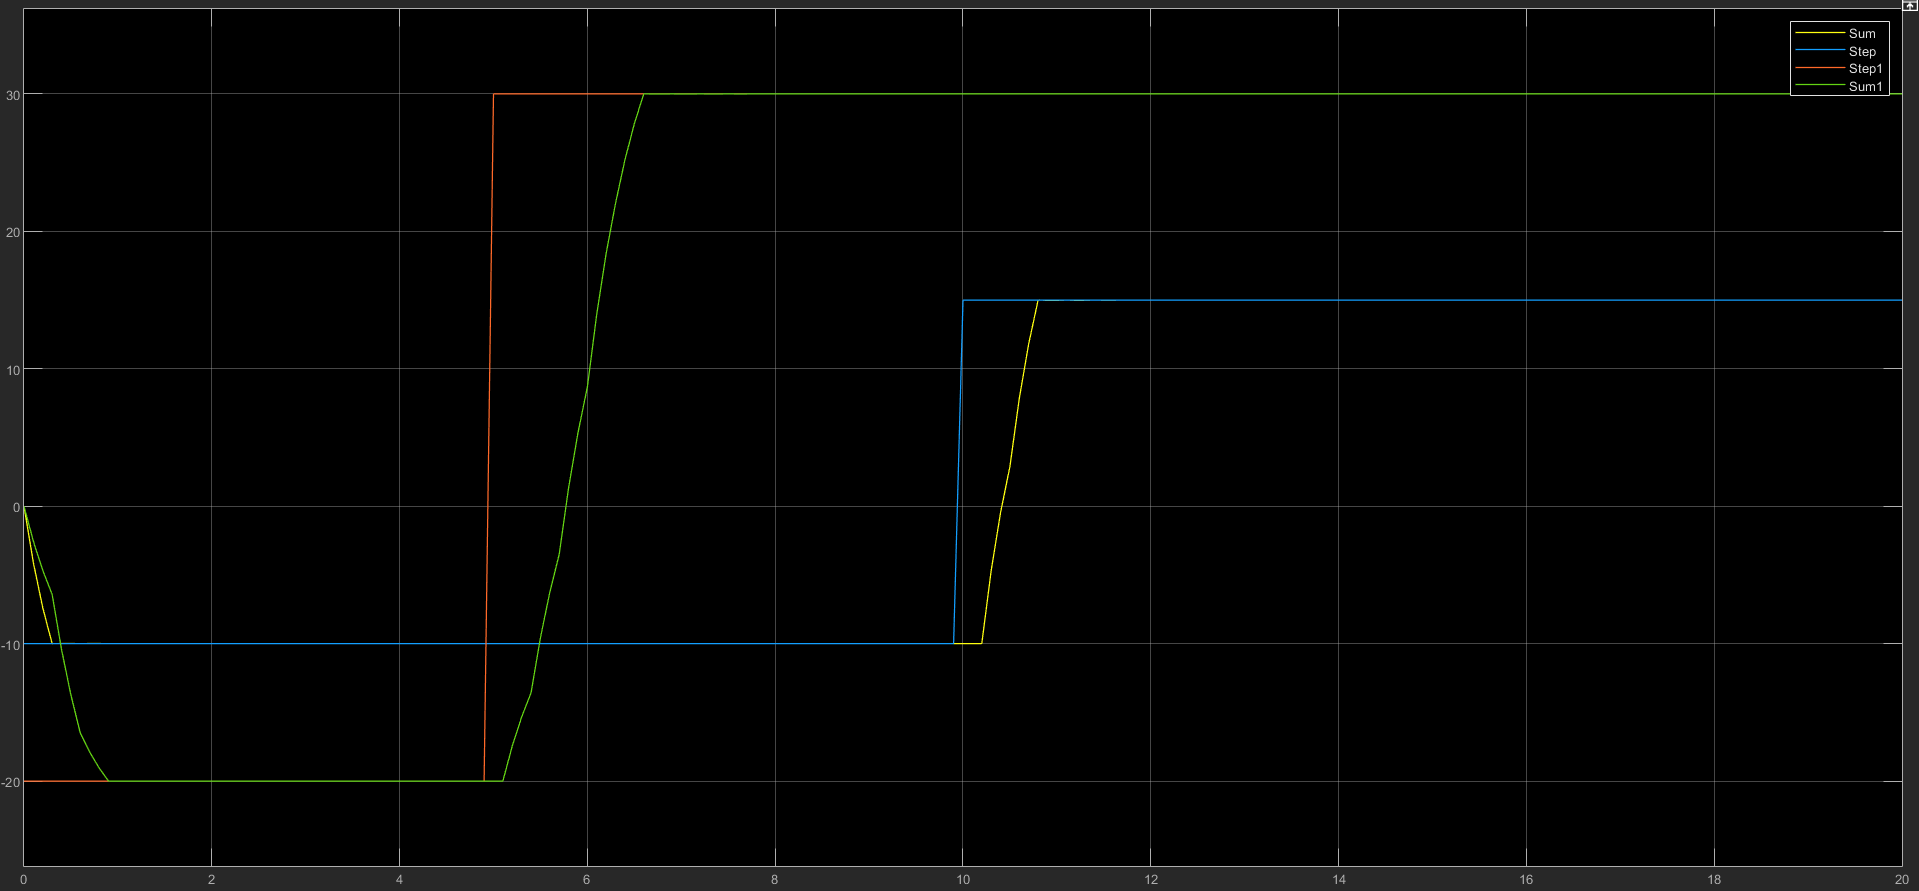
\includegraphics[width=1\linewidth]{../img/Q2_output_updated}
 	\caption{}
 	\label{fig:q2outputupdated}
 \end{figure}
 

\section{پاسخ سوال 3}
\subsection{بخش یکم}
در بخش ابتدایی از این سوال، با در اختیار داشتن ماتریس های حالت سیستم، مدل سیستم را در متلب تعریف کرده و ویژگی های آن را بررسی می کنیم. 
ابتدا قطب ها و صفر های سیستم را مطابق بخش زیر به دست می آوریم:
\[
\text{Poles} = 0, -470.4125, \textcolor{red}{6.7897}, -6.5872
\]

\[
\text{zeros} = -7.1060, 7.1040, 0.0161
\]

مشاهده می شود که این سیستم دارای یک قطب در مبدا و همچنین یک قطب سمت راست است. بنابراین، می توان انتظار داشت که در حالت طبیعی و بدون اعمال کنترلر، سیستم رفتار پایداری نداشته باشد.
این نتیجه را با رسم صفر و قطب های این سیستم نیز می توانیم مشاهده کنیم
\begin{figure}
	\centering
	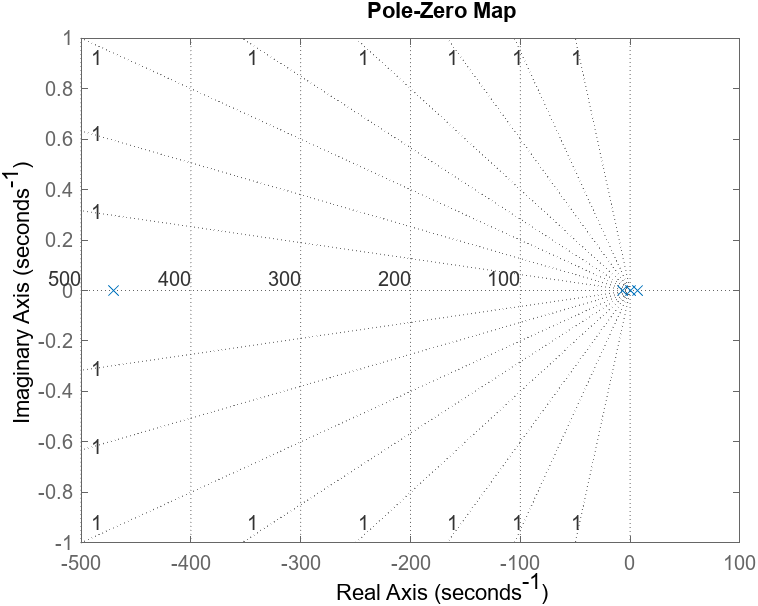
\includegraphics[width=0.7\linewidth]{../img/continues_Poles}
	\caption{}
	\label{fig:continuespoles}
\end{figure}

سپس، برای بررسی رویت پذیری و کنترل پذیری این سیستم، با بررسی رنک ماتریس های زیر می توانیم پاسخ را بیابیم. در صورتی که این ماتریس ها رنک کاملی داشته باشند، آنگاه می توان نتیجه گرفت که کنترل پذیر و یا رویت پذیر هستند. 

با بررسی سیستم مورد استفاده در این قسمت، می بینیم که این ماتریس هم \textbf{رویت پذیر} و هم \textbf{کنترل پذیر} است

پس از به دست آوردن مدل حالت سیستم در بخش قبل، در اینجا آن را به یک مدل گسسته تبدیل می کنیم. برای این کار، با استفاده از دستور
 c2d
  سیستم را گسسته می کنیم. در گام بعد، ماتریس های حالت این سیستم گسسته از مدل برای استفاده های بعدی استخراج می شود. حال، مجددا صفر و قطب های این سیستم را به دست آورده و آنها را رسم می کنیم.
	
\begin{figure}[H]
	\centering
	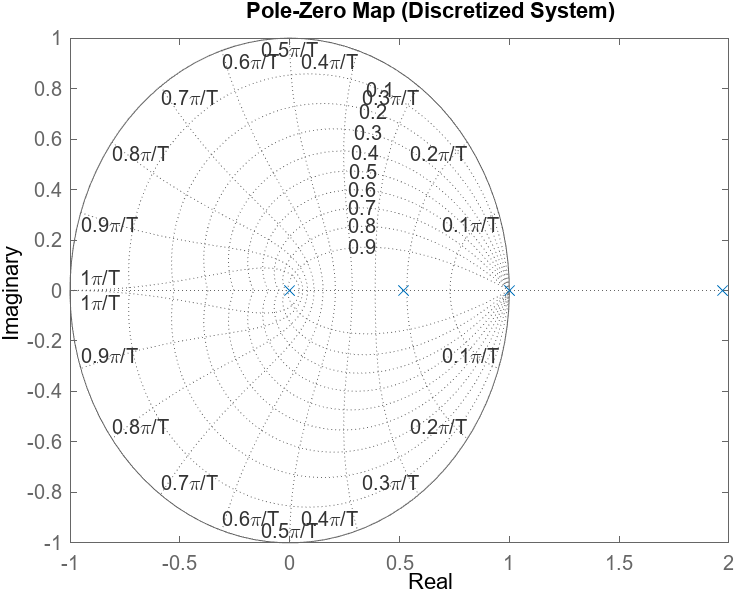
\includegraphics[width=0.7\linewidth]{../img/discrete_Poles}
	\caption{}
	\label{fig:discretepoles}
\end{figure}

در نهایت، پاسخ پله ی این سیستم را رسم می کنیم. اما انتظار داریم که پاسخی ناپایدار به دست بیاید.
\begin{figure}[H]
	\centering
	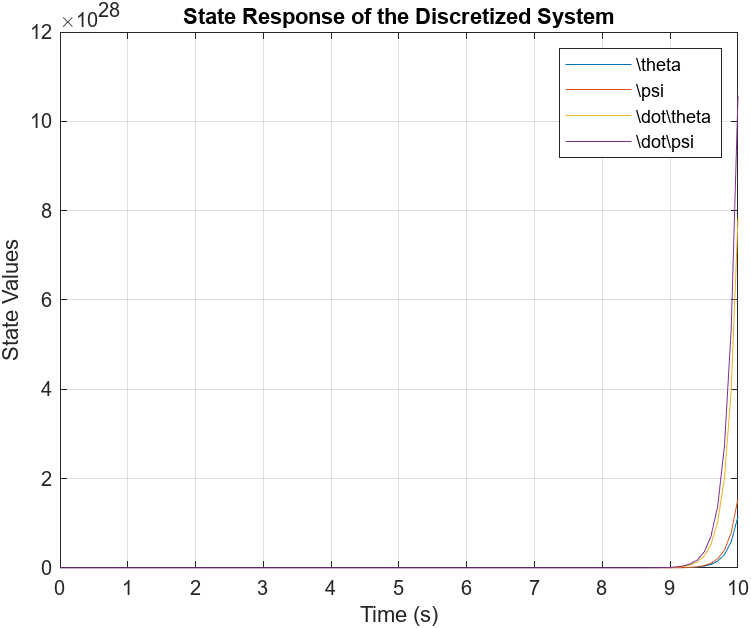
\includegraphics[width=0.9\linewidth]{../img/discrete_response}
	\caption{}
	\label{fig:discreteresponse}
\end{figure}


\subsection{بخش دوم}
	در این بخش، ابتدا سیستم در محیط سیمولینک تعریف شده و برای گام اول، پاسخ حالت صفر آن را نمایش می دهیم. همچنین شرایط اولیه مورد استفاده نیز در حالت اولیه برای بلوک معادلات حالت سیستم لحاظ می شود.
	\[
	x_0 = [0, 0.1, 0, 0]
	\]
	
\begin{figure}[H]
	\centering
	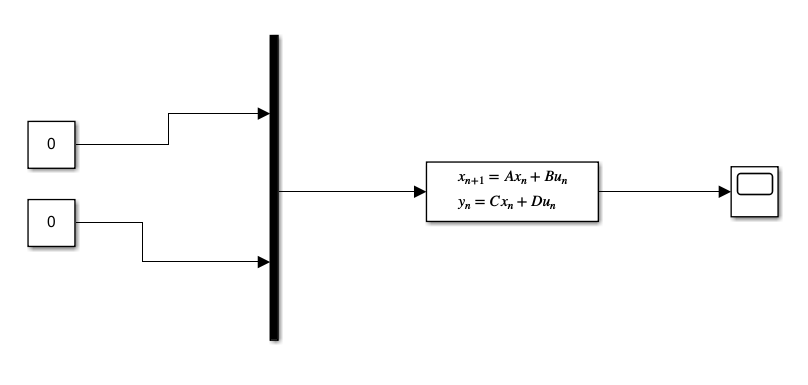
\includegraphics[width=0.7\linewidth]{../img/system_Zero_Responce_Simulink}
	\caption{}
	\label{fig:systemzeroresponcesimulink}
\end{figure}

با اجرای برنامه و مشاهده ی نتیجه ی شبیه سازی، مجددا مشاهده می کنیم که پاسخ سیستم ناپایدار بوده و به بی نهایت میل می کند.
	
 
\begin{figure}[H]
	\centering
	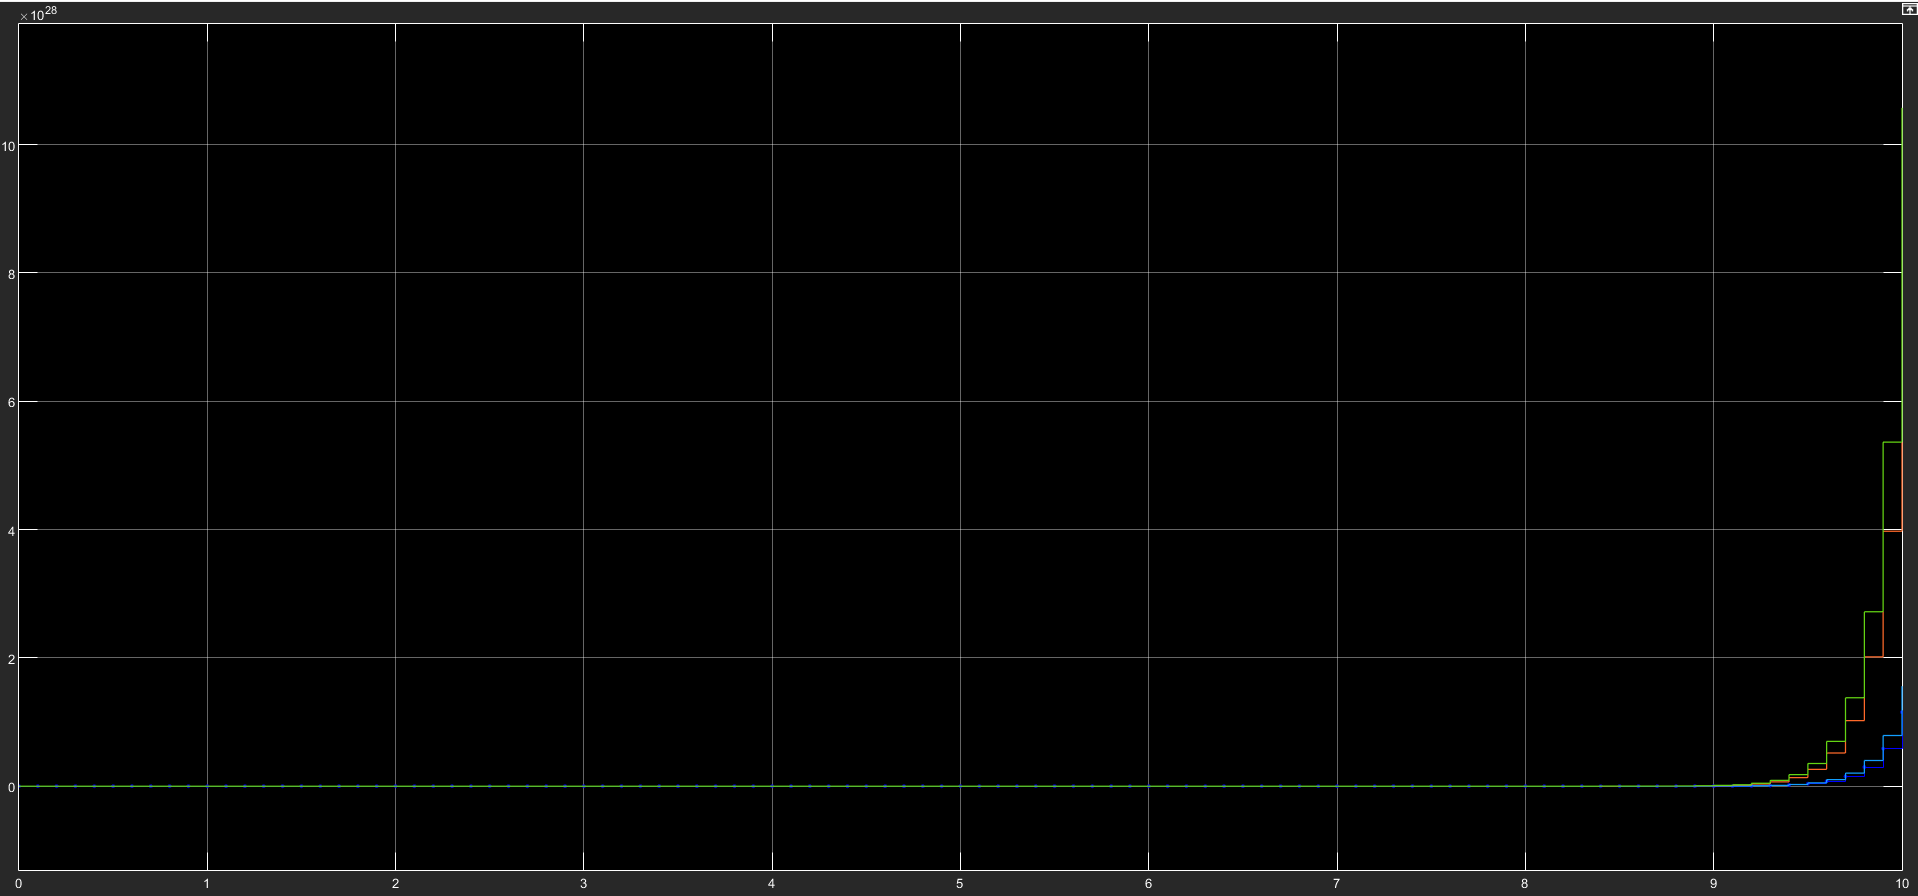
\includegraphics[width=1\linewidth]{../img/Q2_Zero_Response}
	\caption{}
	\label{fig:q3zeroresponse}
\end{figure}
 
 در این مثال و بخش پیشین، بازه زمانی نمونه برداری بر روی 0.1 ثانیه تنظیم شده است.
 
 \subsection{بخش سوم}
 در بخش سوم، بر روی سیستم طراحی شده، دو کنترلر MPC و LQR پیاده سازی می شود. همچنین، اغتشاشی به اندازه ی 0.05 در بازه زمانی بین ثانیه های 4 و 5 به سیستم اعمال می شود. 
 
 \begin{figure}
 	\centering
 	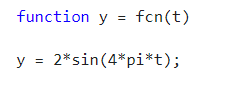
\includegraphics[width=1\linewidth]{../img/Q3_Disturbance}
 	\caption{}
 	\label{fig:q3disturbance}
 \end{figure}
 
 \subsubsection{MPC}
 برای ساخت اغتشاش، از دو بلوک پله با علامت های متفاوت استفاده شده است. بلوک دیاگرام این سیستم در بخش زیر نمایش داده شده است.
 
\begin{figure}[H]
	\centering
	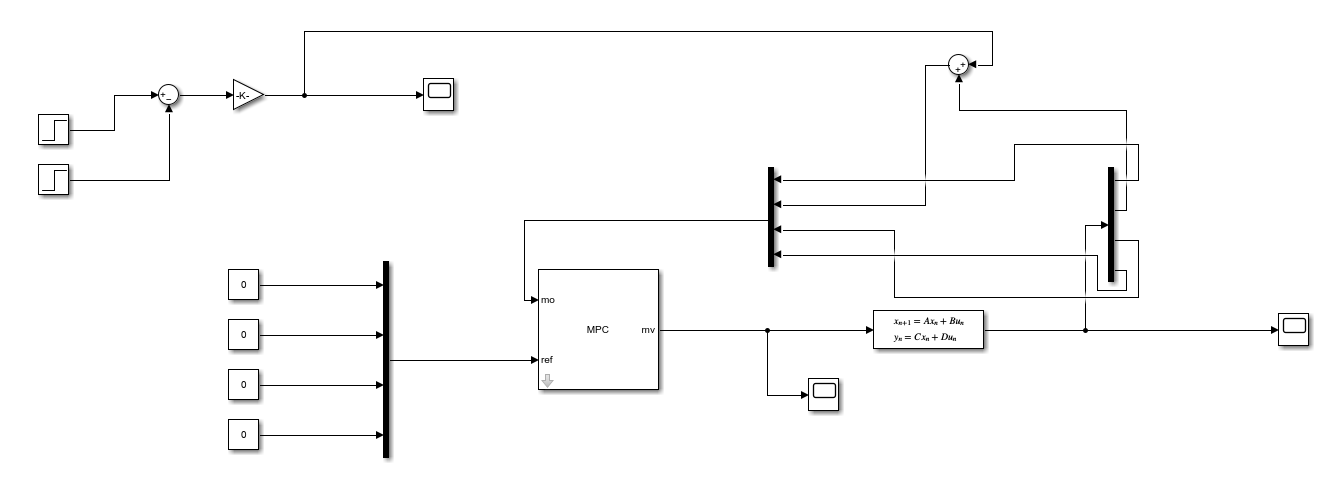
\includegraphics[width=1\linewidth]{../img/Q3_MPC_Block}
	\caption{}
	\label{fig:q3mpcblock}
\end{figure}
 
 تنظیم پارامتر های بلوک کنترلر MPC با مقادیر زیر تنظیم شده است:
 
 \[
 \begin{array}{|c|c|}
 	\hline
 	\textbf{Parameter} & \textbf{Value} \\ 
 	\hline
 	T_s \, (\text{Sampling Time}) & 0.1 \\ 
 	\hline
 	\text{Prediction Horizon} & 20 \\ 
 	\hline
 	\text{Control Horizon} & 10 \\ 
 	\hline
 \end{array}
 \]
 
 با اجرای این برنامه، می توانیم پاسخ های خروجی را به صورت زیر مشاهده کنیم:
 
 
 
\begin{figure}[H]
	\centering
	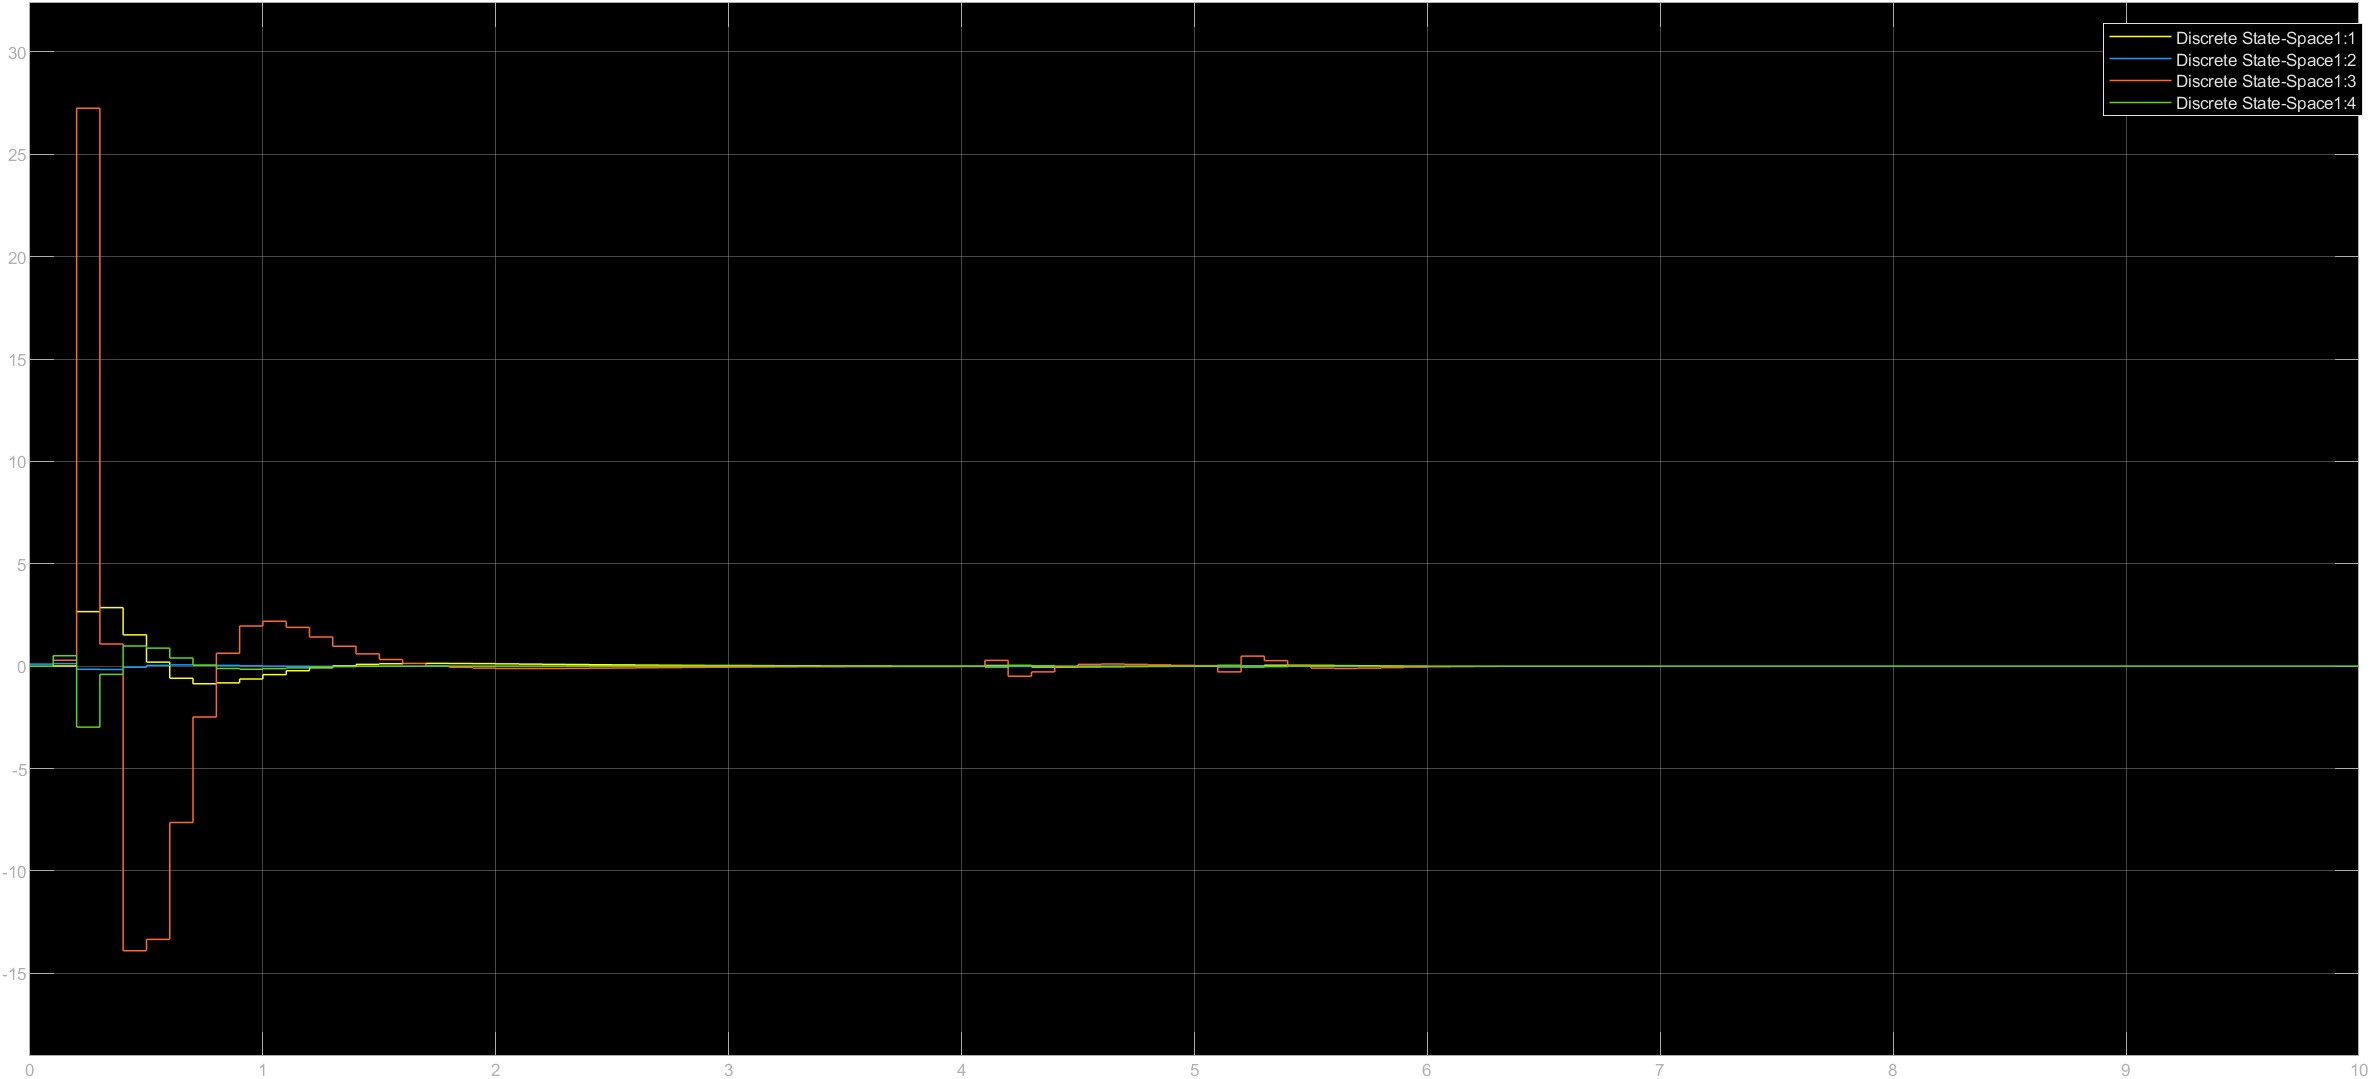
\includegraphics[width=1\linewidth]{../img/Q3_MPC_Output}
	\caption{پاسخ کنترلر MPC}
	\label{fig:q3mpcoutput}
\end{figure}
 
\begin{figure}[H]
	\centering
	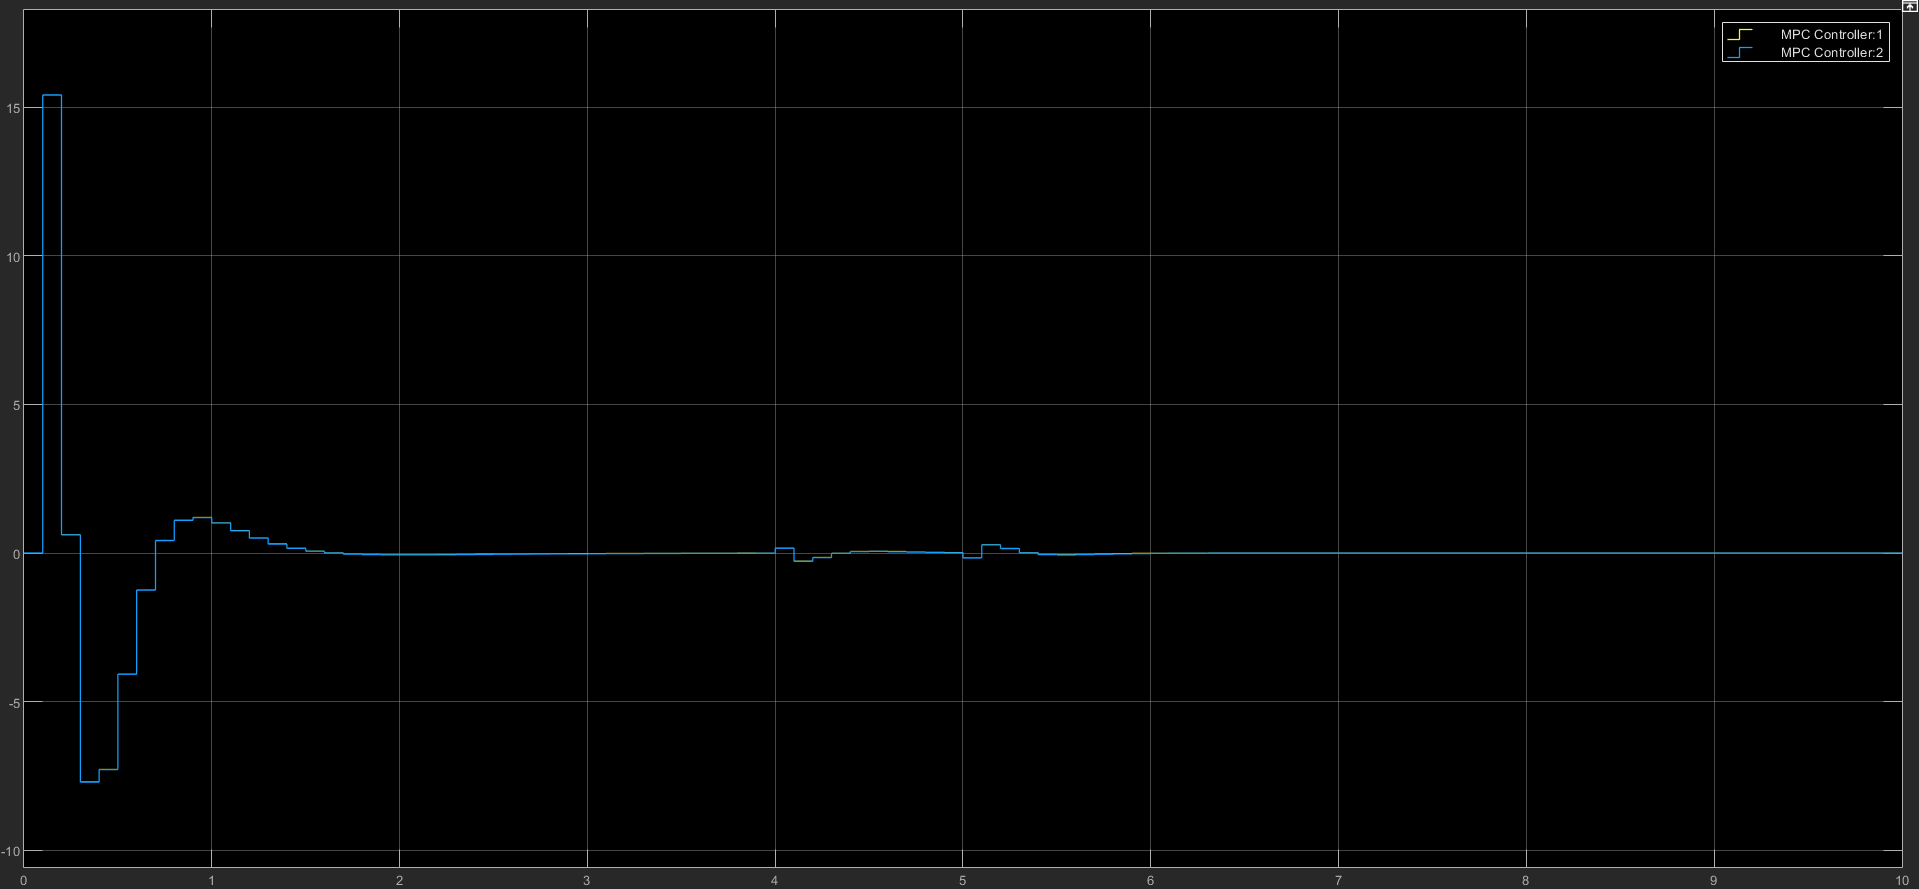
\includegraphics[width=1\linewidth]{../img/Q3_MPC_control_effort}
	\caption{تلاش کنترلی MPC}
	\label{fig:q3mpccontroleffort}
\end{figure}
 
 
 \begin{figure}[H]
 	\centering
 	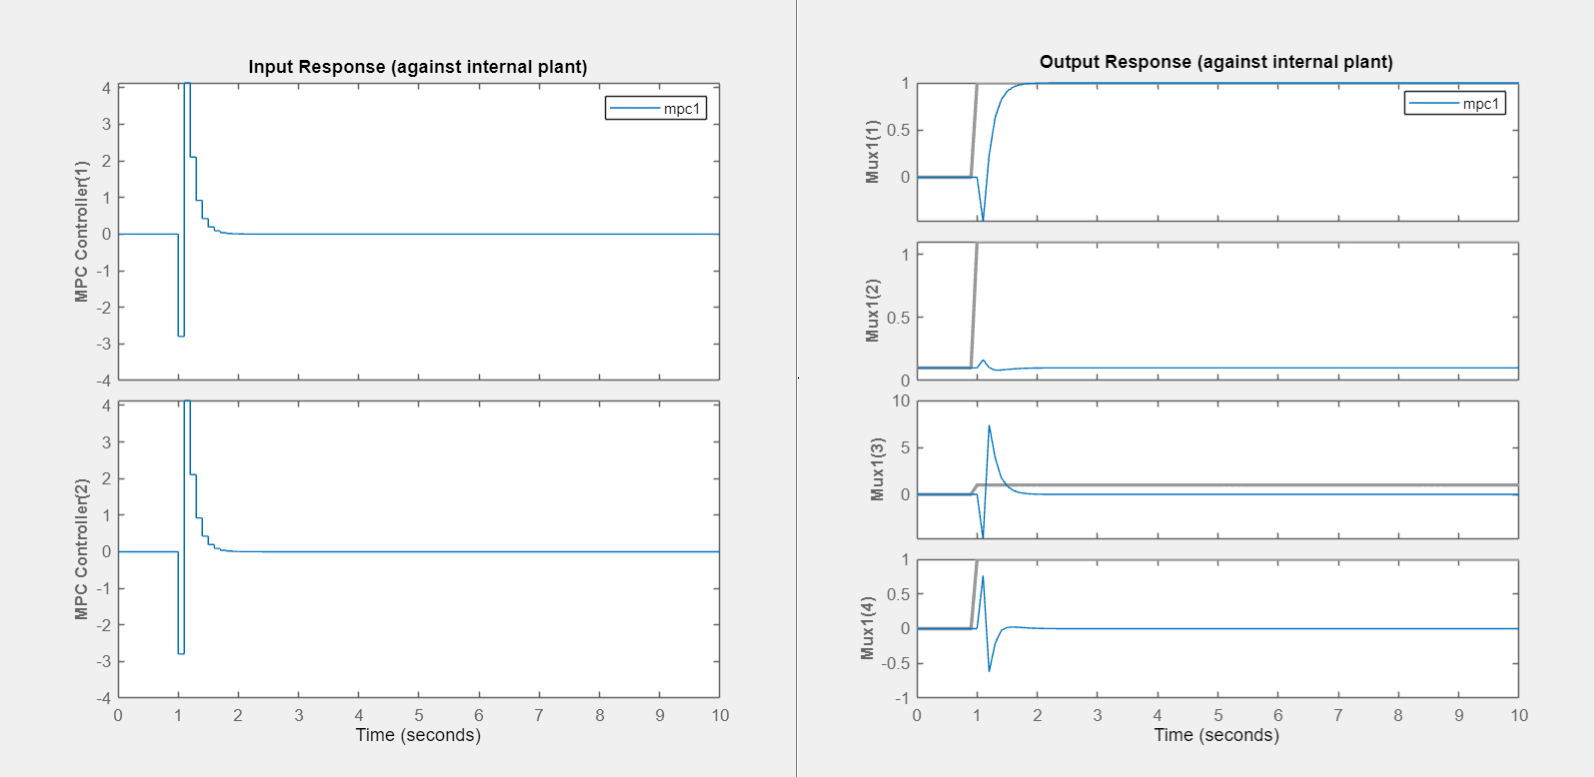
\includegraphics[width=1\linewidth]{../img/Q3_MPC_Setting}
 	\caption{تلاش کنترلی و پاسخ سیستم به ازای هر حالت}
 	\label{fig:q3mpcsetting}
 \end{figure}
 
 چنان که مشاهده می شود، کنترلر MPC مورد استفاده توانسته خروجی های اول و سوم را با میزان خطای قابل قبولی کنترل کند. اما این سیستم برای کنترلر حالت های دوم و چهارم عملکرد مناسبی ندارد و ان چنان که در پاسخ سیستم دیده می شود، در صورت اعمال اغتشاش به خروجی دوم، فراجهش زیادی در پاسخ دریافت خواهیم کرد.
 
 \subsubsection{LQR}
 پ
 برای طراحی و پیاده سازی کنترلر LQR، لازم است یک ماتریس بهره در فیدبک حالت ضرب شود. پیش از پیاده سازی این کنترلر در محیط سیمولینک، با استفاده از مدل سیستم گسسته، پارامتر های مورد نیاز برای محاسبه ی مقادیر این بهره به دست می آید. برای این منظور، با استفاده از دو ماتریس A و B و همچنین تعریف دو ماتریس جدید R و Q، می توانیم بهره را به دست بیاوریم. 
 با استفاده از دستور dlqr، پارامترهای LQR به صورت زیر به دست می آید.
 
\[
k_{LQR} = 
\begin{bmatrix}
	-0.7434 & -60.6744 & -1.0184 & -8.0624 \\
	-0.7434 & -60.6744 & -1.0184 & -8.0624
\end{bmatrix}
\]

\[
s_{LQR} = 
1.0 \times 10^{5} \cdot
\begin{bmatrix}
	0.0067 & 0.0793 & 0.0014 & 0.0111 \\
	0.0793 & 2.1697 & 0.0381 & 0.3005 \\
	0.0014 & 0.0381 & 0.0008 & 0.0053 \\
	0.0111 & 0.3005 & 0.0053 & 0.0418
\end{bmatrix}
\]

\[
p_{LQR} = 
\begin{bmatrix}
	0.7348 + 0.0000i \\
	0.4950 + 0.0215i \\
	0.4950 - 0.0215i \\
	-0.0000 + 0.0000i
\end{bmatrix}
\]

 
 با قرار دادن مقدار به دست آمده برای K در بلوک کنترلی طراحی شده برای این سیستم که در قسمت پایین نمایش داده شده است، می توانیم برنامه را اجرا کنیم:
 
 \begin{figure}[H]
 	\centering
 	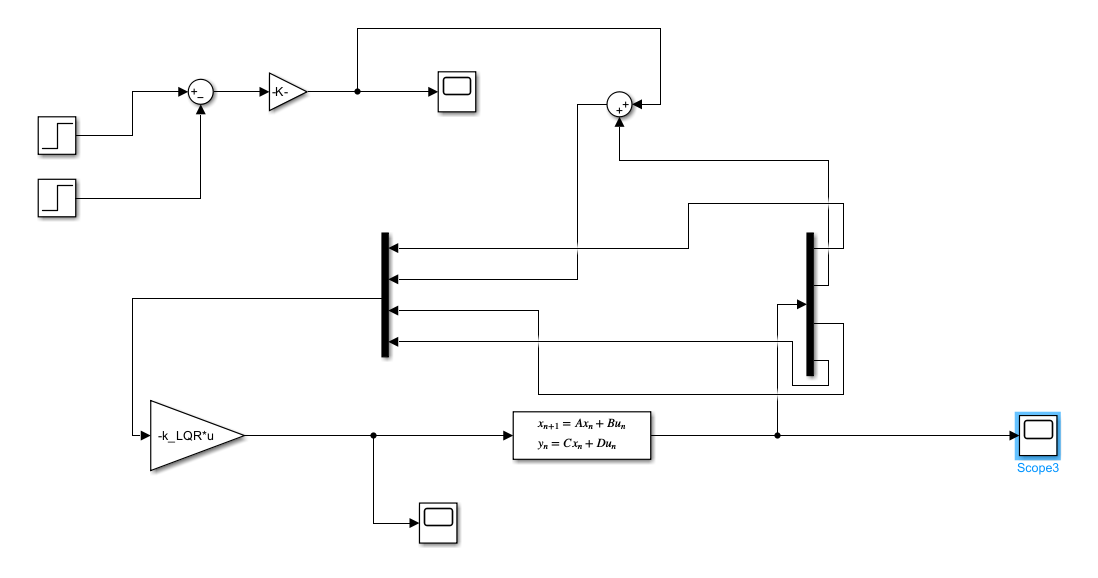
\includegraphics[width=1\linewidth]{../img/Q3_LQR_Block}
 	\caption{بلوک دیاگرام کنترلر LQR}
 	\label{fig:q3lqrblock}
 \end{figure}
 
 \begin{figure}[H]
 	\centering
 	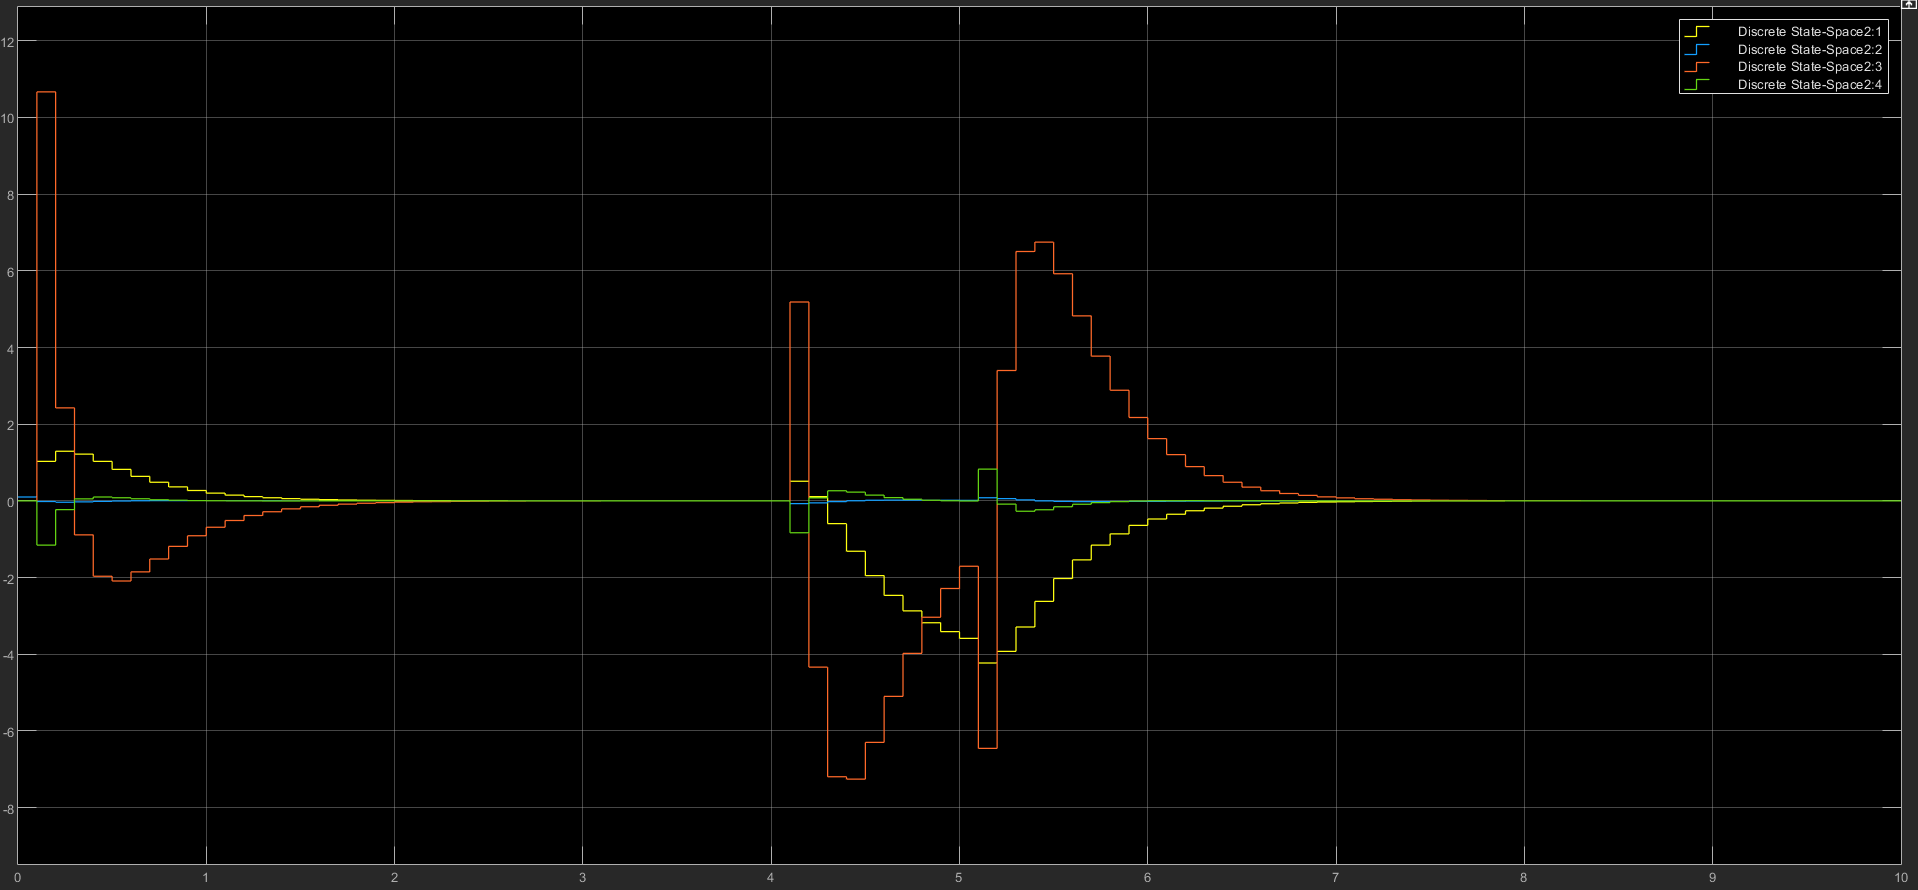
\includegraphics[width=1\linewidth]{../img/Q3_LQR_Output}
 	\caption{پاسخ کنترلر LQR}
 	\label{fig:q3lqroutput}
 \end{figure}
 
 \begin{figure}[H]
 	\centering
 	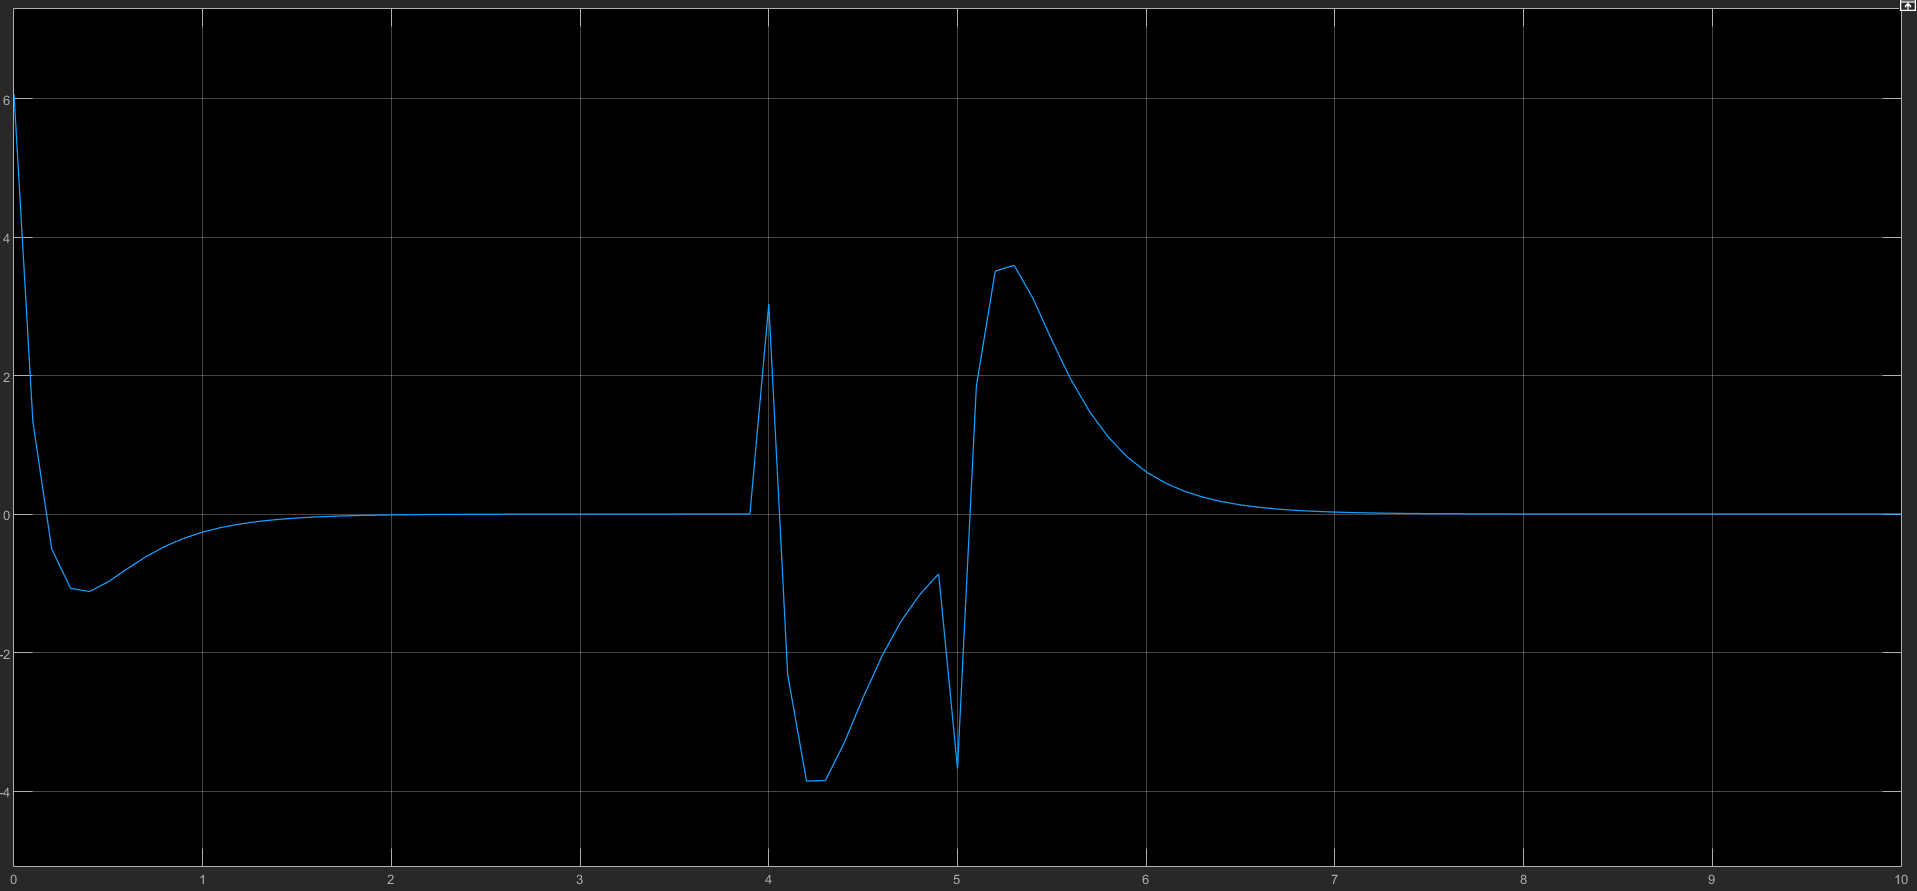
\includegraphics[width=1\linewidth]{../img/Q3_LQR_control_effort}
 	\caption{تلاش کنترلی LQR}
 	\label{fig:q3lqrcontroleffort}
 \end{figure}
 
 مشاهده می شود که این کنترلر نیز می تواند مانند کنترل MPC، خروجی را کنترل کند. با این حال، عملکرد کنترلر در کنترل حالت دوم نتایج قابل قبولی ندارد.
 
\subsection{بخش چهارم}

در این بخش، با لحاظ کردن محدودیت بر روی خروجی اول سیستم در دو حالت سخت و نرم، رفتار سیستم را بررسی می کنیم.
محدودیت این قسمت به صورت زیر تعریف می شود.
\[
-0.3 \leq \theta \leq 1.5
\]

\subsubsection{سخت}

با تنظیم محدودیت ها و اجرای برنامه در حالت سخت خواهیم داشت:
\begin{figure}[H]
	\centering
	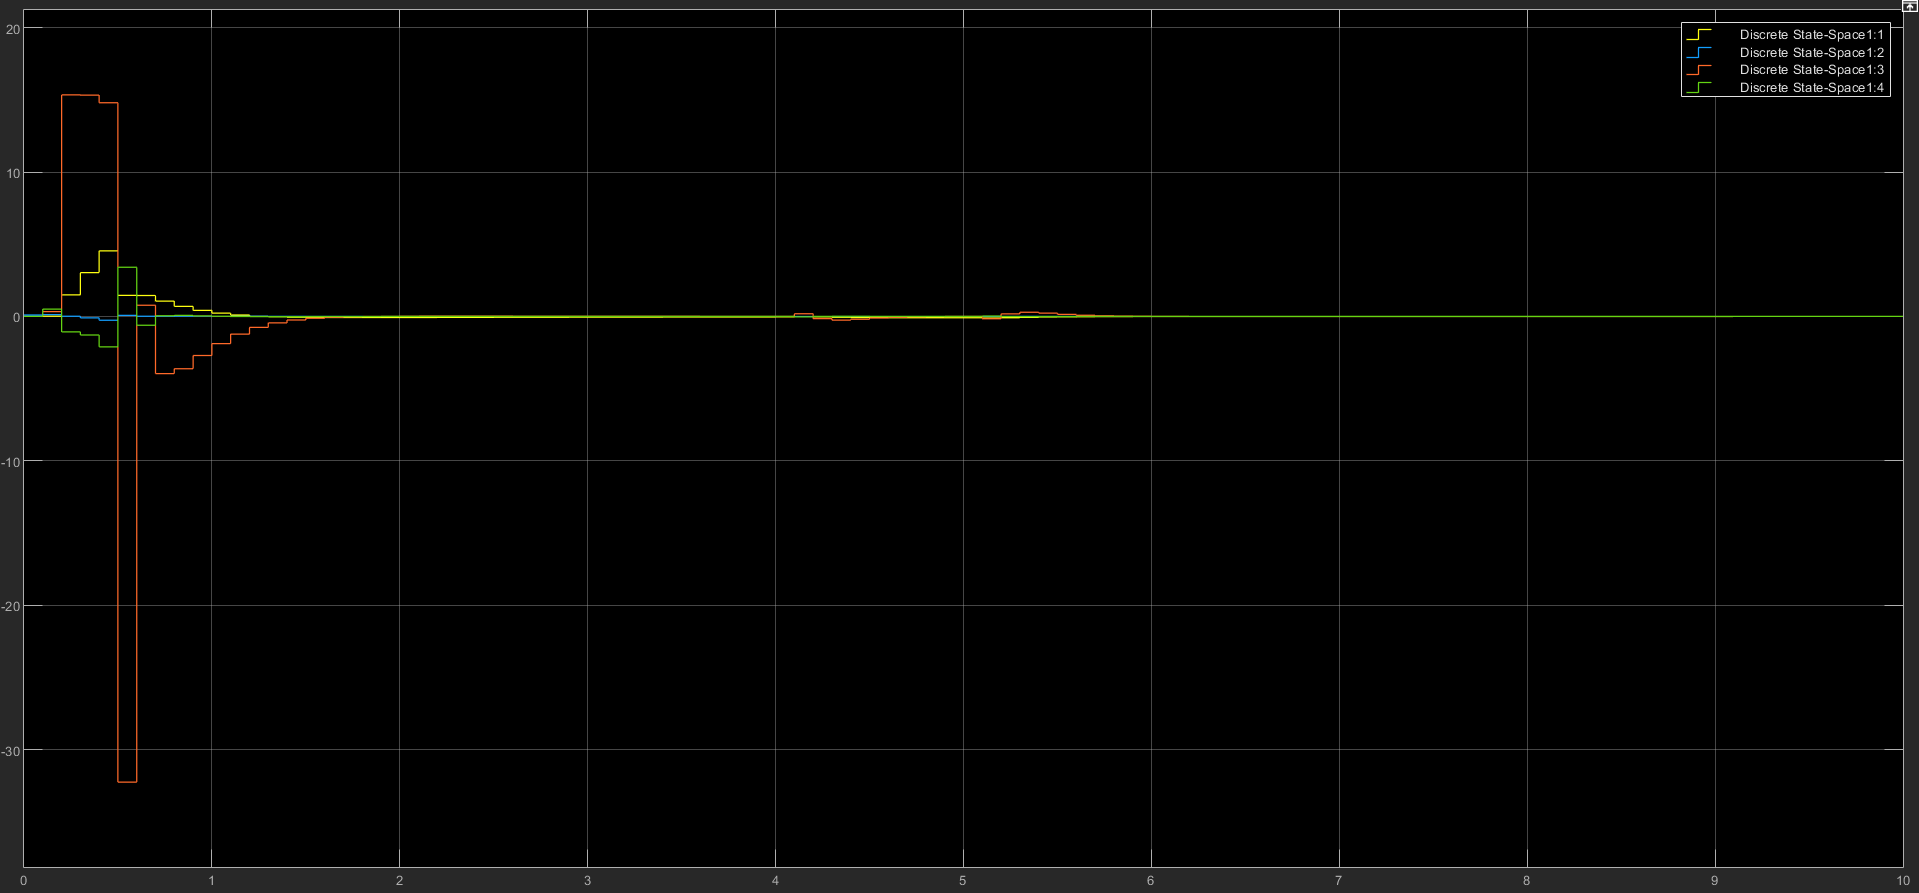
\includegraphics[width=1\linewidth]{../img/Q4_Hard_Output}
	\caption{پاسخ کنترلر MPC محدود با قید های سخت}
	\label{fig:q4hardoutput}
\end{figure}

\begin{figure}[H]
	\centering
	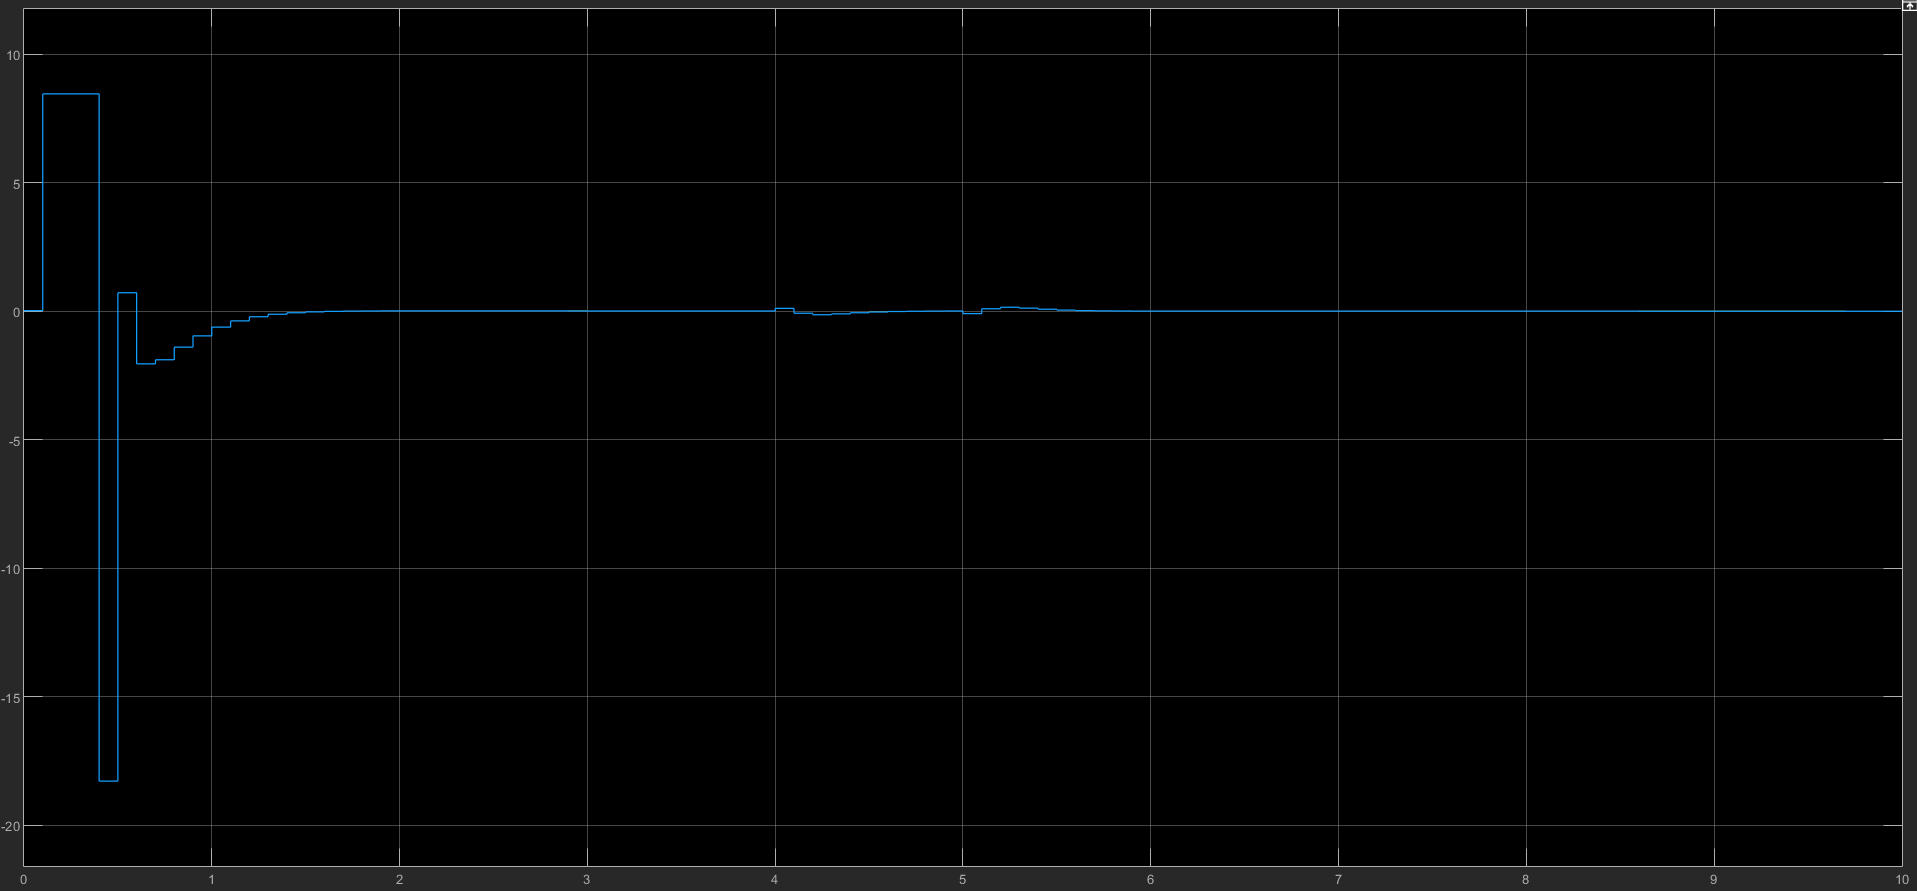
\includegraphics[width=1\linewidth]{../img/Q4_Hard_control_effort}
	\caption{تلاش کنترلی کنترلر MPC با قید های سخت}
	\label{fig:q4hardcontroleffort}
\end{figure}

\subsubsection{نرم}
با تنظیم محدودیت ها و اجرای برنامه در حالت نرم خواهیم داشت:
\begin{figure}[H]
	\centering
	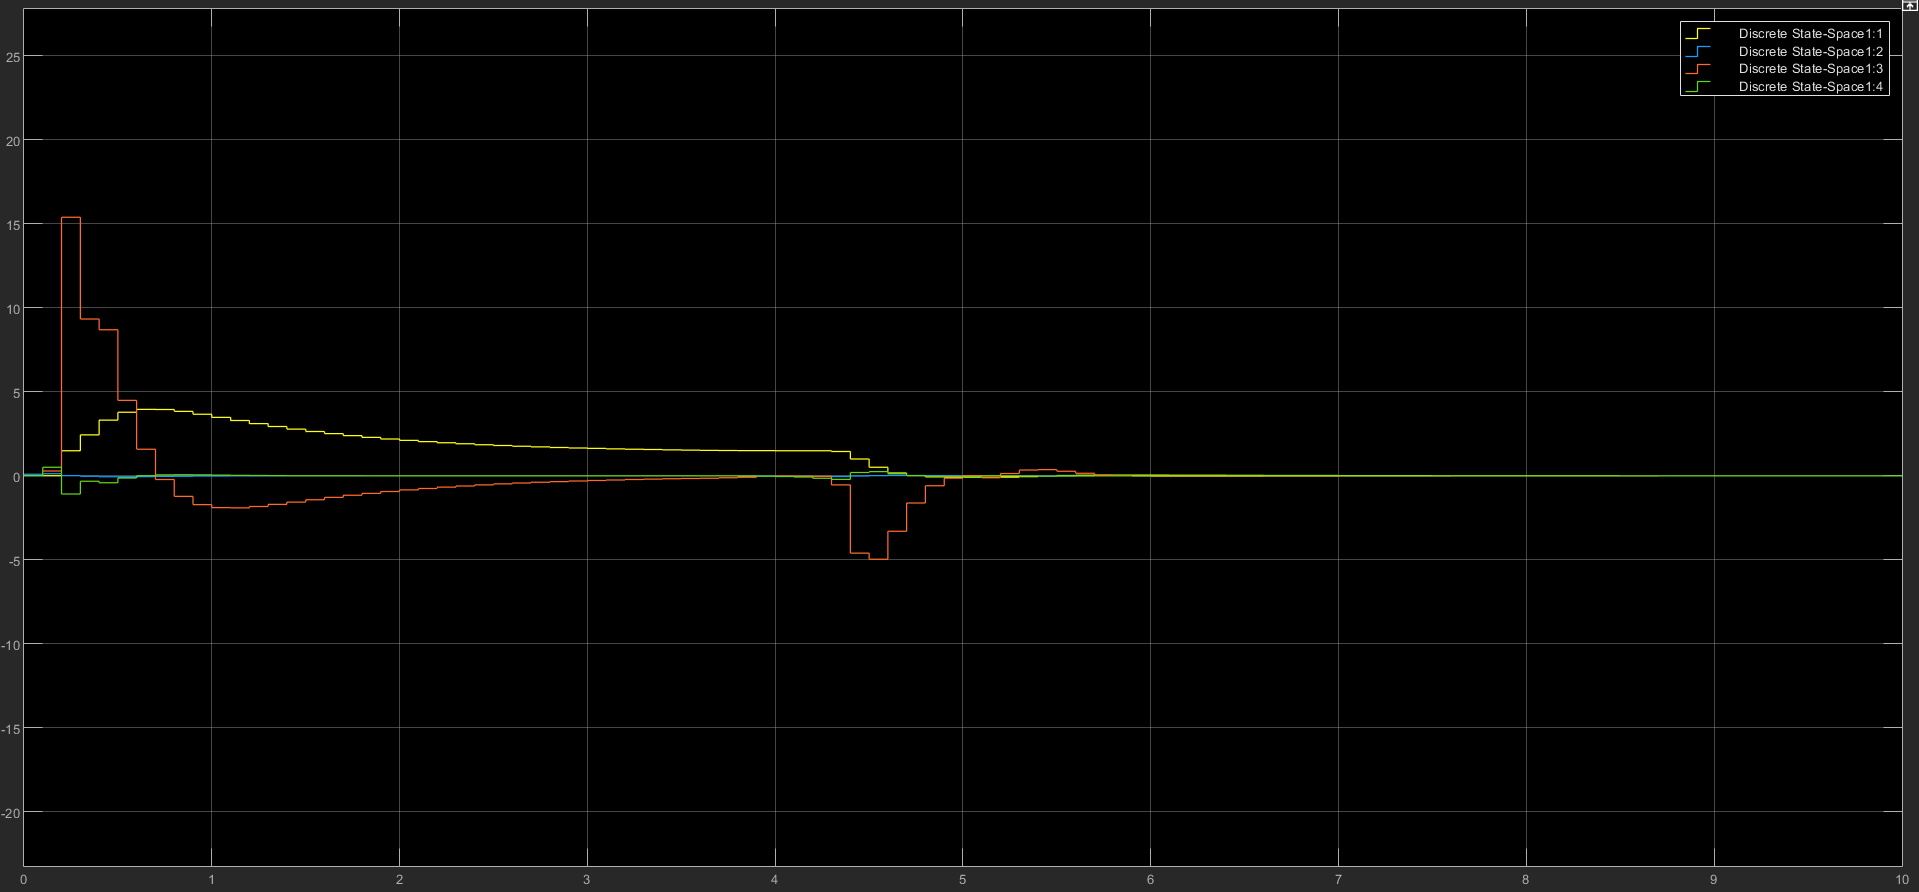
\includegraphics[width=1\linewidth]{../img/Q4_Soft_output}
	\caption{پاسخ کنترلر MPC محدود با قید های نرم}
	\label{fig:q4softoutput}
\end{figure}

\begin{figure}[H]
	\centering
	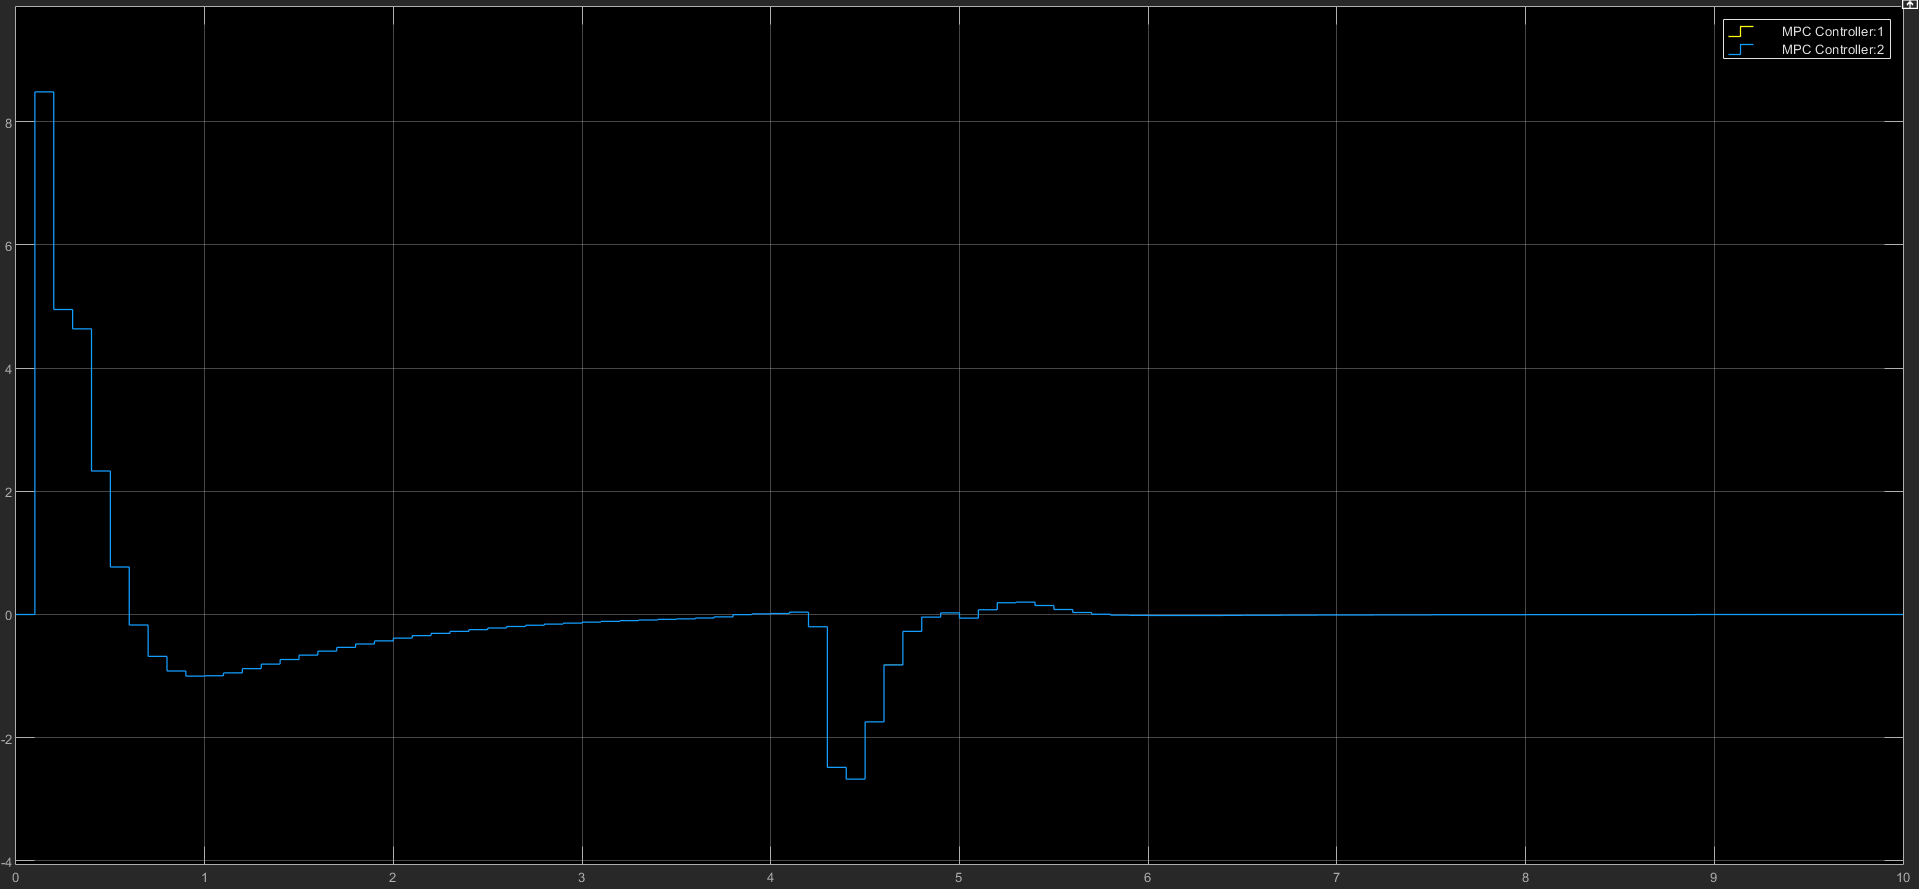
\includegraphics[width=1\linewidth]{../img/Q4_Soft_control_effort}
	\caption{تلاش کنترلی کنترلر MPC با قید های نرم}
	\label{fig:q4softcontroleffort}
\end{figure}

\subsection{بخش پنجم}
\subsubsection{نرم}
با تنظیم محدودیت ها و اجرای برنامه در حالت نرم خواهیم داشت:

\begin{figure}[H]
	\centering
	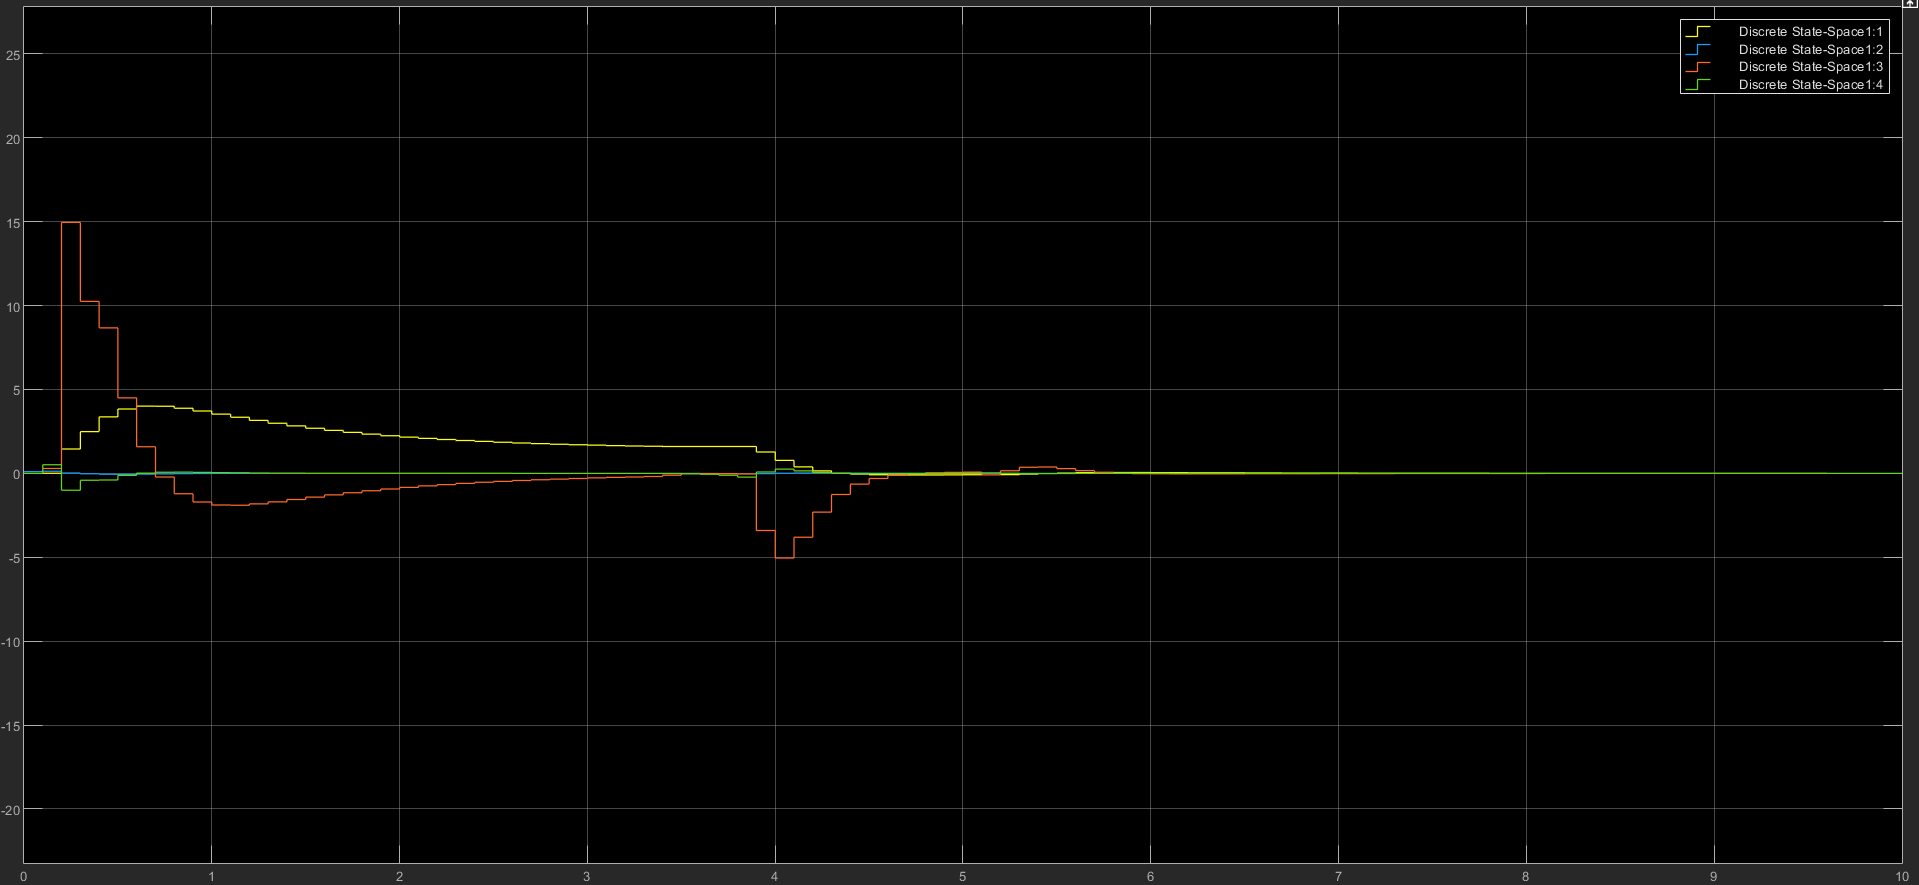
\includegraphics[width=1\linewidth]{../img/Q5_Soft_output}
	\caption{تلاش کنترلی کنترلر MPC با قید های نرم}
	\label{fig:q5softoutput}
\end{figure}

\begin{figure}[H]
	\centering
	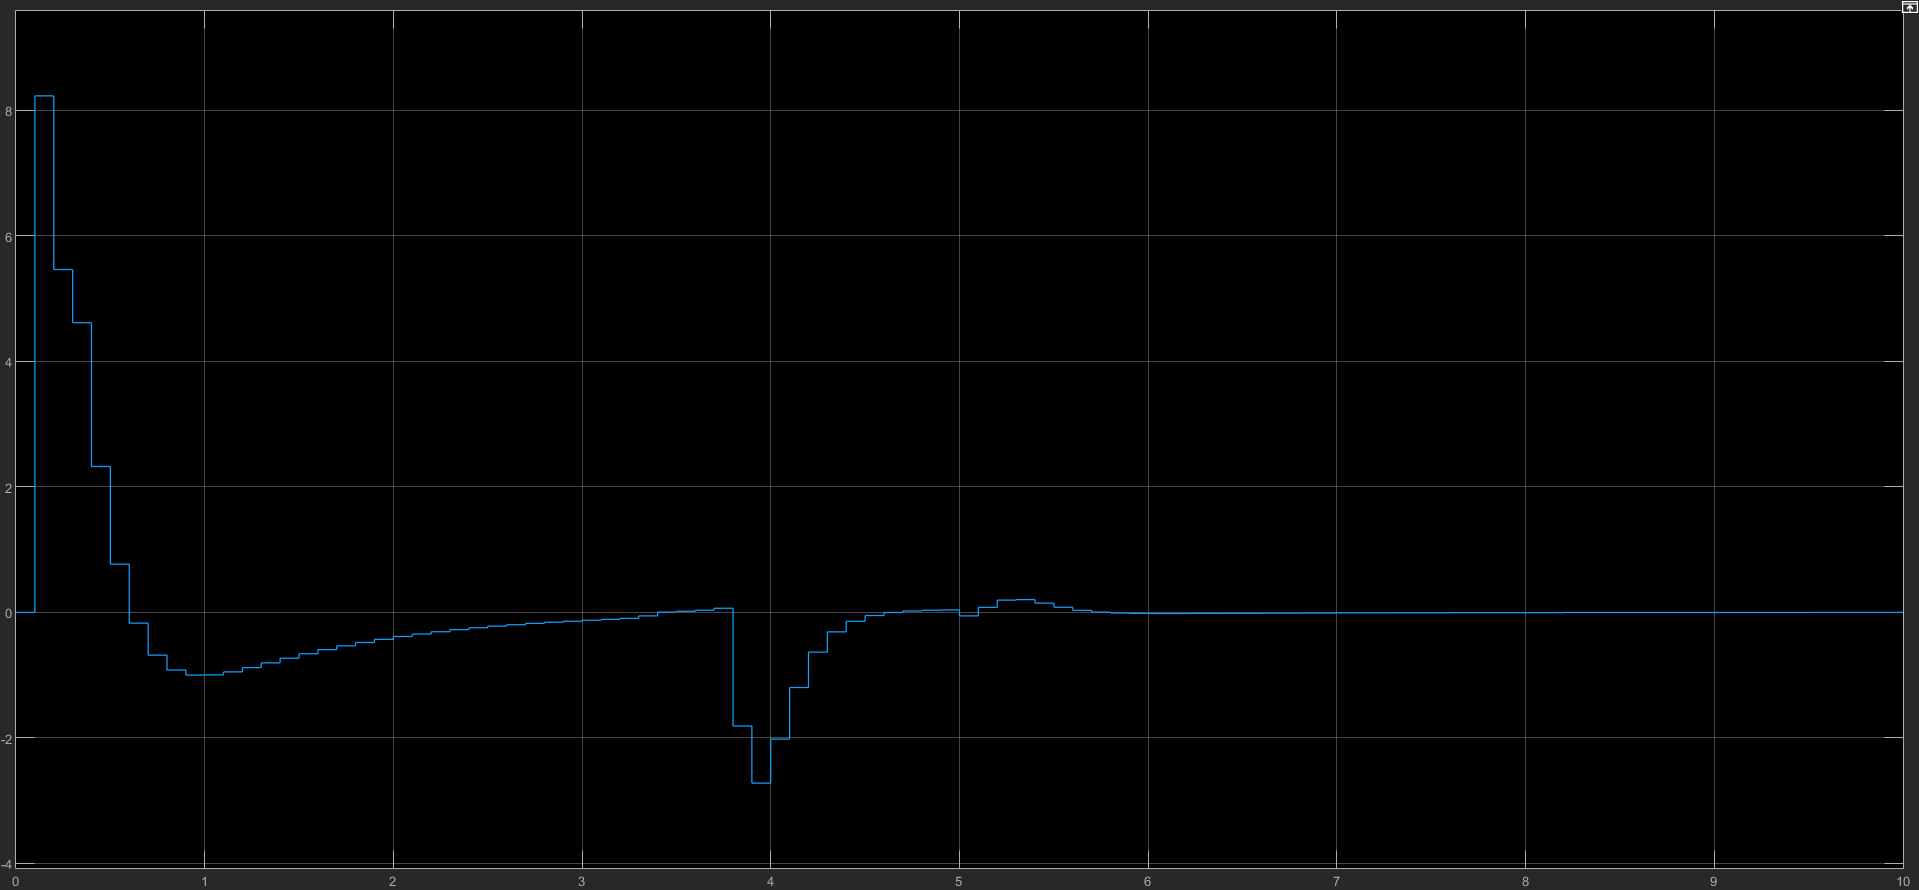
\includegraphics[width=1\linewidth]{../img/Q5_Soft_control_effort}
	\caption{پاسخ کنترلر MPC محدود با قید های نرم}
	\label{fig:q5softcontroleffort}
\end{figure}

\subsubsection{سخت}
با تنظیم محدودیت ها و اجرای برنامه در حالت سخت خواهیم داشت:

\begin{figure}[H]
	\centering
	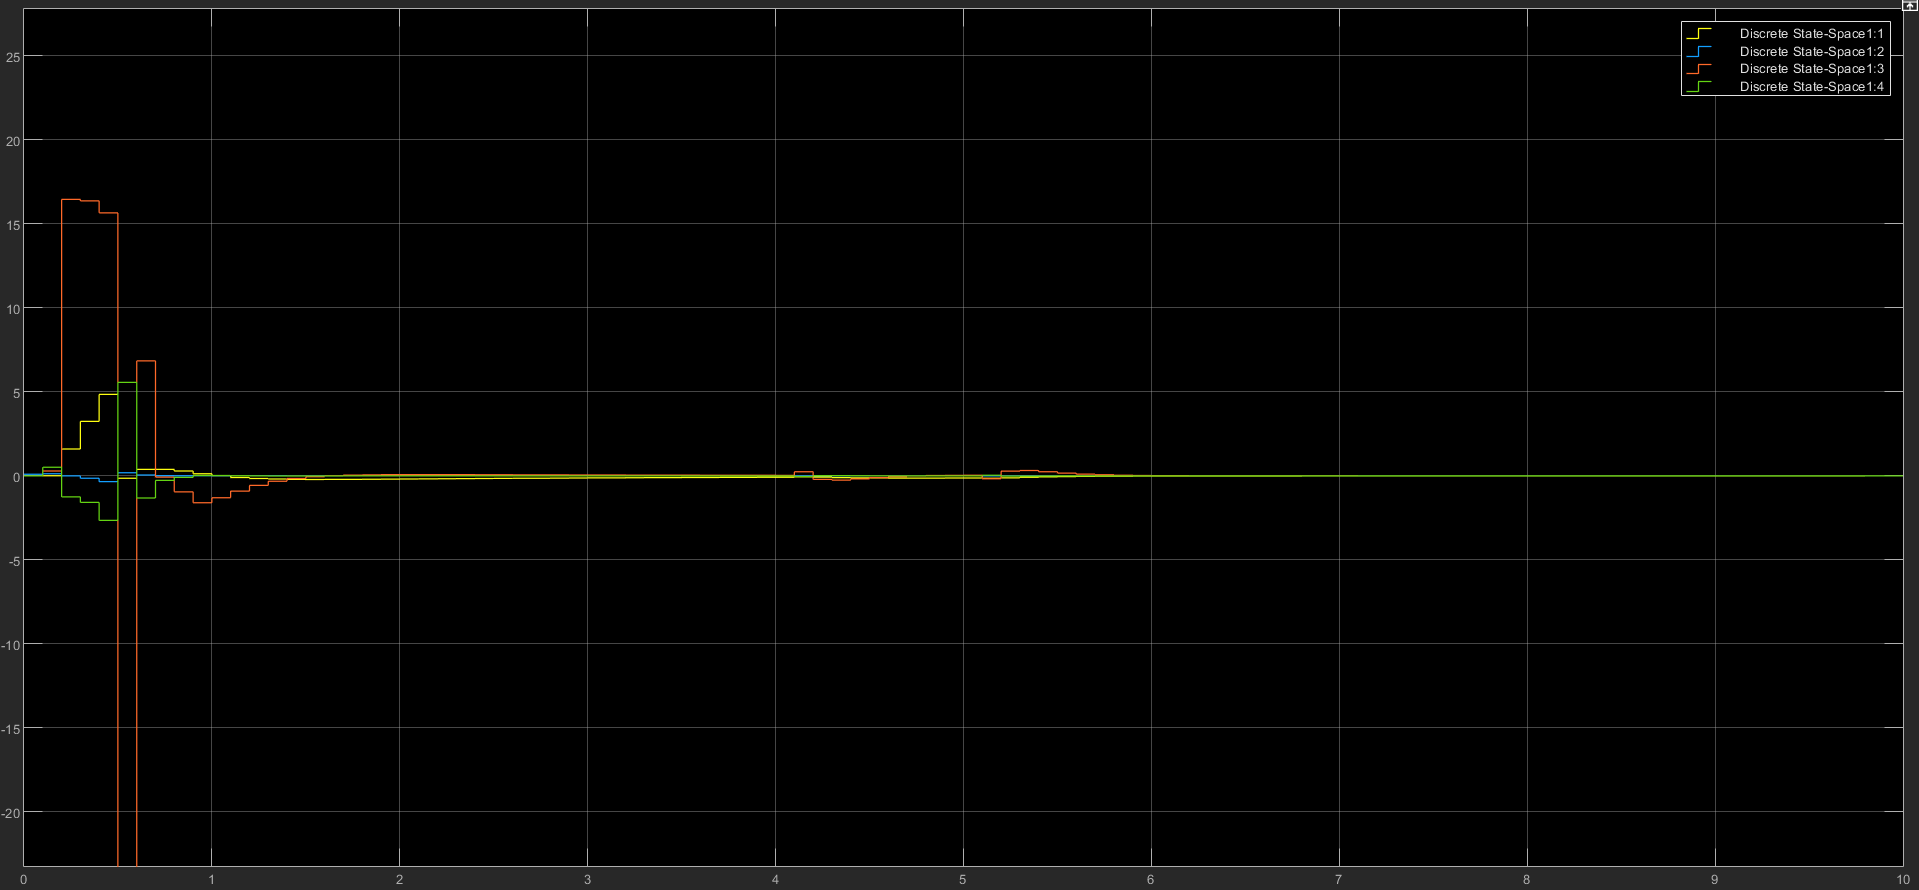
\includegraphics[width=1\linewidth]{../img/Q5_Hard_output}
	\caption{پاسخ کنترلر MPC محدود با قید های سخت}
	\label{fig:q5hardoutput}
\end{figure}

\begin{figure}[H]
	\centering
	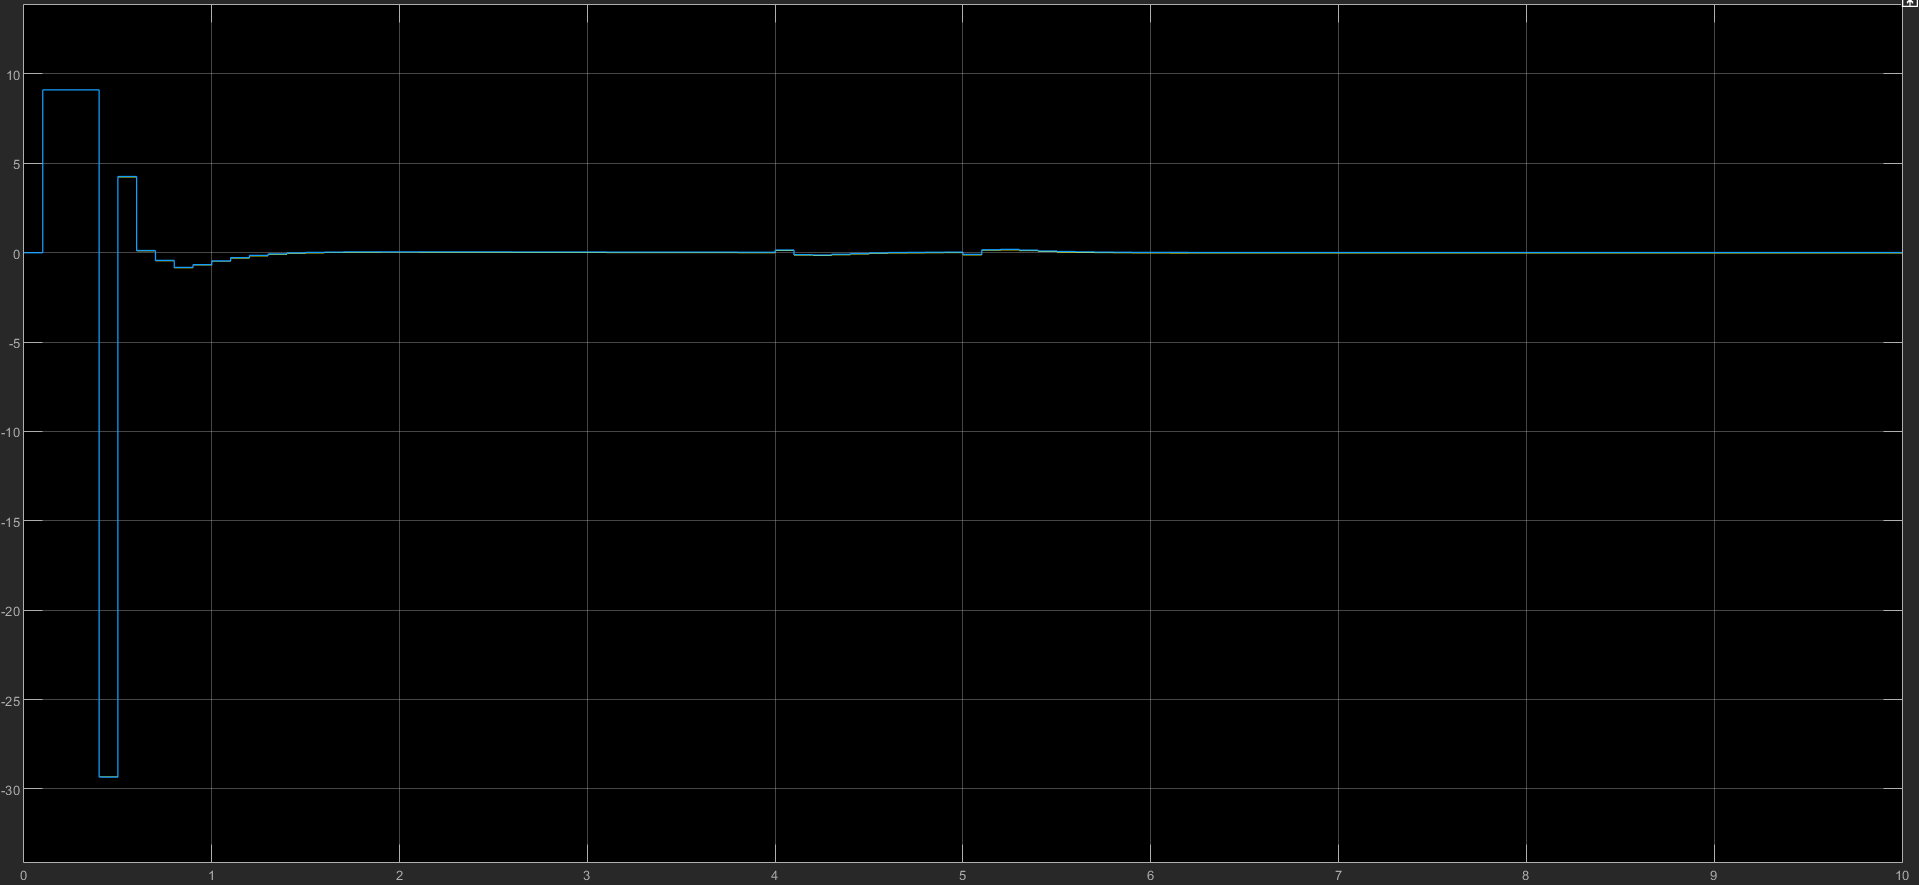
\includegraphics[width=1\linewidth]{../img/Q5_Hard_control_effort}
	\caption{پاسخ کنترلر MPC محدود با قید های سخت}
	\label{fig:q5hardcontroleffort}
\end{figure}



 
 
 
 
 
 
 
 
 
 
 